\documentclass[11pt]{article}
\usepackage{graphicx}
\usepackage{biblatex}
\usepackage{booktabs}
\usepackage{tabularx}
\usepackage[percent]{overpic}
\usepackage{placeins}
\usepackage{amsmath}

\title{Evaluation of LoRa Mesh Networks in an Urban Environment}
\author{
NSERC USRA Final Report\\
Jonathan Earle\\
}
\date{August 2026}

\addbibresource{usra_2026_final_report.bib}

\begin{document}

\maketitle

\section{Abstract}

LoRa mesh networks are becoming increasingly popular for Internet of Things (IoT) communication. In particular, the open-source firmware Meshtastic has grown in popularity amongst hobbyists, with some claiming it has potential as an emergency network when internet services are down. This project evaluates the effectiveness of Meshtastic in an urban environment through various range, latency, and routing experiments conducted using a LoRa mesh testbed deployed across the Dalhousie University campus. Simulations were also performed to determine the performance of networks on a city-wide scale while comparing simulated and real-world results. Test results show that building obstructions significantly impede device range, indicating that nodes should be placed on adjacent streets which act as propagation corridors. Reliable zero-hop communication was achieved at a range of approximately 260 meters and up to 1.1km on an adjacent street. Although the campus deployment exhibited reliable multi-hop communication on a small scale, simulations show that a Meshtastic network covering Halifax would experience severe performance limitations, with network reach peaking at 54\% before congestion and message delay increase considerably.

\section{Introduction}

Amateur radio is a unique hobby that dates back to around 1914, when the American Radio Relay League was founded by Hiram Percy Maxim \cite{the_national_association_for_amateur_radio_ham_nodate}. Today, there are an estimated three million licensed ham radio operators \cite{clash_ham_nodate}; thus, it is clear that an old hobby that uses dated technology is not fading. One of the main appeals of amateur radio is that users can easily communicate in the event of an emergency when internet services fail. Now, with the rapid growth of the Internet of Things, two unrelated topics are colliding. LoRa has grabbed the attention of amateur radio hobbyists, as, like ham radio, it is a wireless communication technique that requires little preexisting infrastructure. This has resulted in a massive community of LoRa mesh enthusiasts, building a plethora of software and firmware that allow anyone with an inexpensive LoRa radio to communicate over several kilometers. The most notable of these firmware systems is Meshtastic.

Meshtastic is an open-source, decentralized mesh networking system that uses LoRa to enable off-grid communication over long distances. Meshtastic is easy to use and accessible to everyone. Because LoRa operates on unlicensed frequency bands, anyone can start using Meshtastic as long as they have access to a cheap LoRa radio and a computer to flash firmware. Because of its accessibility, Meshtastic has a large, growing community that continually pushes new firmware updates and additional software.

Meshtastic firmware operates on inexpensive, low-power microcontrollers equipped with a LoRa radio module. Most devices use ESP32 chips with Semtech’s SX126x or SX127x transceiver series \cite{smartnmagic_meshtastic_nodate}. Depending on the hardware, devices can connect to a Meshtastic node in three ways: USB serial, Bluetooth, or an IP network via Wi-Fi or Ethernet \cite{meshtastic_overview_nodate}. There are a variety of interfaces for a device to connect to a Meshtastic node. The most common connection method is Bluetooth using the Meshtastic Mobile app; however, there is also a Meshtastic web client and a Meshtastic command-line interface. Using these interfaces, one can send text messages, GPS, device telemetry, and other small pieces of data over LoRa either directly to users or to channels \cite{meshtastic_portnum_nodate}. Users can also modify their device settings using their interface of choice \cite{meshtastic_webflasher_nodate}. However, settings like region and modem preset must be identical for successful communication.

Before use, the region setting must be applied. This setting determines the frequency range, duty cycle and power limit, ensuring compliance with regional laws \cite{meshtastic_initial_nodate}. To simplify settings for users, Meshtastic encapsulates LoRa settings, such as spreading factor and bandwidth, under “modem presets”. The modem preset name is based on the range and data rate. The default modem preset is LONG\_FAST and is used by most of the community \cite{meshtastic_radio_nodate}. 

Meshtastic text communication occurs either through direct messaging or through channels. Every device has one primary channel and can add more channels later \cite{meshtastic_channel_nodate}. Periodic broadcasts such as device telemetry and position are broadcast on this primary channel. Channels have a name and an encryption key. Devices must share the encryption key to communicate in the channel. Unlike channels that use a pre-shared key, direct messages are more secure as they use public-key cryptography \cite{meshtastic_encryption_nodate}. Direct messages also differ from channels in terms of routing logic \cite{meshtastic_mesh_algorithm}.

What makes Meshtastic distinct from other LoRa mesh ecosystems, like MeshCore, is its simple routing protocol. Meshtastic focuses on flooding, in which, when a message is sent, nodes that hear it automatically retransmit. Meshtastic uses ‘managed flooding’, which takes flooding and adds a few more rules \cite{meshtastic_mesh_algorithm}. One of these rules is a hop limit, meaning that a single packet can only be retransmitted a certain number of times \cite{meshtastic_mesh_algorithm}. Another is the suppression of duplicates: packets that have been recently heard (stored in the duplicate cache) will not be relayed \cite{meshtastic_mesh_algorithm}. The final major rule is that sender nodes will prioritize receiver nodes with lower SNR values by giving them a shorter wait time before rebroadcasting. Direct messages use next-hop routing. This means that the first message to the recipient will be managed flooding, but if the message is successful, the node that relayed the message most recently will be denoted as ‘next-hop’ for each node in the path to the recipient. Future messages to the recipient node will always attempt to send to the next-hop node at least three times before falling back to managed flooding, as illustrated in Figure~\ref{fig:managedflooding} \cite{meshtastic_mesh_algorithm}. 

\begin{figure}[htbp]
    \centering
    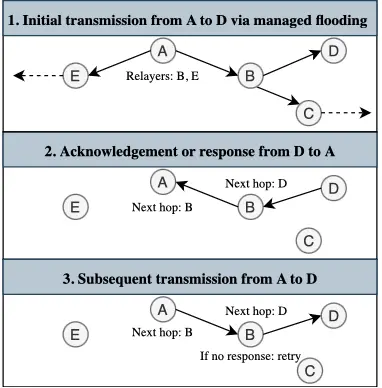
\includegraphics[width=0.7\linewidth]{images/image20.png}
    \caption{Meshtastic Managed Flooding Protocol}
    \label{fig:managedflooding}
\end{figure}

The downside of a mesh, especially one that uses flooding, is that each transmission occupies more airtime. Consequently, increasing the number of nodes has a compounding negative effect on performance. Therefore, it is easy for a Meshtastic network to become oversaturated. Although Meshtastic is indeed a mesh network, nodes can be given specific roles. For example, ROUTER nodes can only relay messages, while CLIENT\_MUTE nodes can only send messages \cite{meshtastic_device_nodate}.

Meshtastic is similar to traditional radio in its use case. It is a communication method that does not rely on the internet or preexisting infrastructure. What gives it an advantage over ham radio is that it does not require a license and that it is inexpensive. Some of the most popular LoRa radios can be found for as little as \$30 \cite{lilygo_t-beam_nodate}. Thus, the main use case is for long-range communication where there is no internet service. Because of the adaptive nature of the meshes and managed flood routing, nodes do not have to remain stationary. Thus, Meshtastic is a good solution for off-grid communication while doing activities like hiking or skiing. Many enthusiasts enjoy the idea of having Meshtastic as a local emergency fail-safe when internet services are down \cite{piputi_meshtastic_2025}. However, it is unknown at what scale Meshtastic is feasible for such communication, especially in an urban area. 

\section{Project Overview}

The goal of this project was to determine the effectiveness of LoRa mesh networks in an urban environment. Because LoRa meshes require little pre-existing infrastructure, it is difficult to maximize their range. Unlike cellular networks, which have elevated towers and large antennas to extend range, the placement of small LoRa radios is relative to the user and the space they have access to. Additionally, to maximize effective communication between LoRa radios, there should be a clear line of sight between nodes. Both of these factors are serious constraints in cities, and the complexity of building shapes and materials in a metropolitan environment makes it difficult to deploy these networks or predict their performance. 

Achieving the project goal is not a simple task and cannot be addressed by just one test. This project consists of a variety of tests, all using or simulating Meshtastic devices to collect various performance metrics and benchmarks and form hypotheses. The project began with a simple range test and evolved into more complex tests using a campus Meshtastic deployment. This data was compared to Meshtastic simulations, some of which attempted to predict the behaviour of a Halifax-wide deployment. Effectiveness is difficult to define as many different metrics could be used to evaluate performance. Some metrics include network reach, message relay, average range between nodes, collision rate and latency. It is also difficult to quantify at what point effectiveness is achieved, as it depends on the use case; for example, what percentage of network reach shows sufficient connectivity.

\begin{table}[htbp]
    \centering
    \caption{Default Meshtastic settings used during experiments.}
    \label{tab:default-settings}
    \begin{tabularx}{\textwidth}{lX}
        \toprule
        \textbf{Setting} & \textbf{Value} \\
        \midrule
        Device Role & CLIENT \\
        Modem Preset & LONG\_FAST \\
        Bandwidth & 250 kHz \\
        Spreading Factor & SF11 \\
        Coding Rate & 4/5 \\
        Max Hops & 3 \\
        TX Power & 20 dBm (T-Beam maximum) \\
        Region & US \\
        Frequency Band & 902--928 MHz (915 MHz ISM band) \\
        Center Frequency & 906.875 MHz \\
        Frequency Slot & 0 (automatic) \\
        Ignore MQTT Packets & false \\
        OK to MQTT & false \\
        Override Duty-Cycle Limit & false \\
        Boosted RX Gain & false \\
        \bottomrule
    \end{tabularx}
\end{table}

\FloatBarrier
\section{Test Procedure and Results}
\subsection{Meshtastic Range Testing}

This was the first set of tests within the internship period. The goal of these tests was to establish a baseline for the range and effectiveness of zero-hop communication between two LoRa mesh radios within an urban environment. Many range tests were conducted in various parts of Halifax and at different scales. For each test, there was one central, stationary LoRa radio receiving packets, while another radio was moving and sending packets. Packet data was collected and stored at the receiving end, and various metrics including distance, RSSI, SNR and latency were measured. All radios used were LILYGO T-Beam v1.2.

\FloatBarrier
\subsubsection{SMU Range Test}

The first range test was conducted at the Saint Mary’s University (SMU) football field and the surrounding campus. The goal of this test was to determine the change in performance as the sending node was taken behind a set of buildings, yet still within some proximity to the receiving node. The test was also used to determine the effectiveness of the RF propagation software, including Radio Mobile and CloudRF, within an urban environment.

Within this testing period, there were three groups of tests, with three tests in each group. Each test group varied in node elevation and distance, while the tests within each group varied in LoRa configuration. The first two tests were conducted within the vicinity of the football field, while the third test was conducted around the entire SMU campus. For each test group, the LoRa preset was set to either SHORT\_TURBO, MEDIUM\_FAST or LONG\_FAST. 

For all tests, a stationary receiver node was placed at the center of the SMU football field while the sender node was mobile, held by someone walking. For the first group of tests, the person holding the sender node would take one lap around the football field and the receiving node was set on the ground. The second group of tests was identical to the first, except the receiving node was elevated approximately 1 meter above the ground. For the third group of tests, the receiving node was again elevated to 1 meter. However, instead of walking around the football field, the participant would begin on Gorsebrook Avenue and walk the closest possible outdoor path on campus to the football field.

\begin{figure}[htbp]
    \centering
    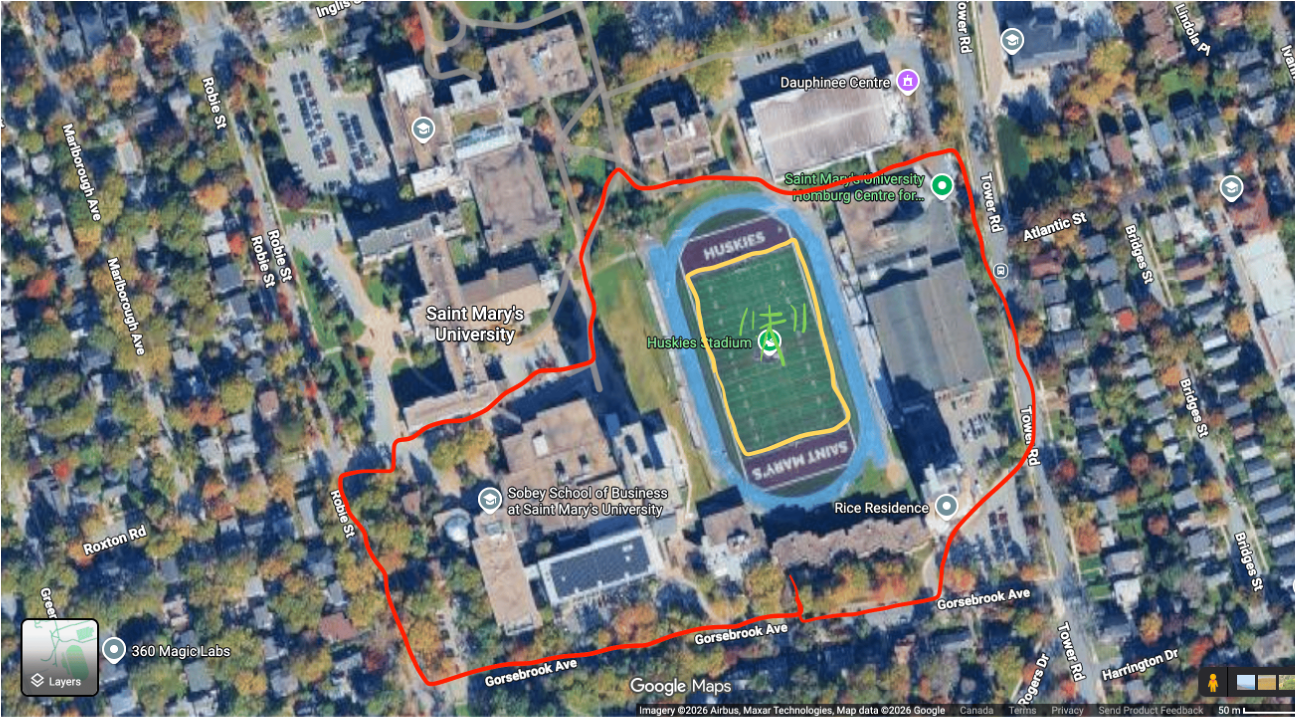
\includegraphics[width=0.7\linewidth]{images/image18.png}
    \caption{SMU Range Test Routes}
    \label{fig:smu_rangetest_route}
\end{figure}

As there was not sufficient time to conduct all experiments, only LoRa settings SHORT\_TURBO and LONG\_FAST were used for each test group. The football field tests showed higher RSSI/SNR values when the receiving node was elevated. Tests in which the node was taken around campus showed a consistent connection in both settings; however, there was a significant drop in both RSSI and SNR when the node was taken onto Robie St., behind the Sobey School of Business, seen in Figure~\ref{fig:smu_rangetest_rssi} and Figure~\ref{fig:smu_rangetest_snr}. This shows that going behind even one building can have a significant impact on zero-hop performance. It also conveys the importance of obtaining a strong line of sight or propagation corridor between all nodes when designing an effective LoRa mesh network. SNR values were generally poorer among all SHORT\_TURBO tests compared to LONG\_FAST ones. RSSI did not change much between LoRa settings. All tests showed that RF software overestimated the potential range of LoRa radios on such settings.

\begin{figure}[htbp]
    \centering
    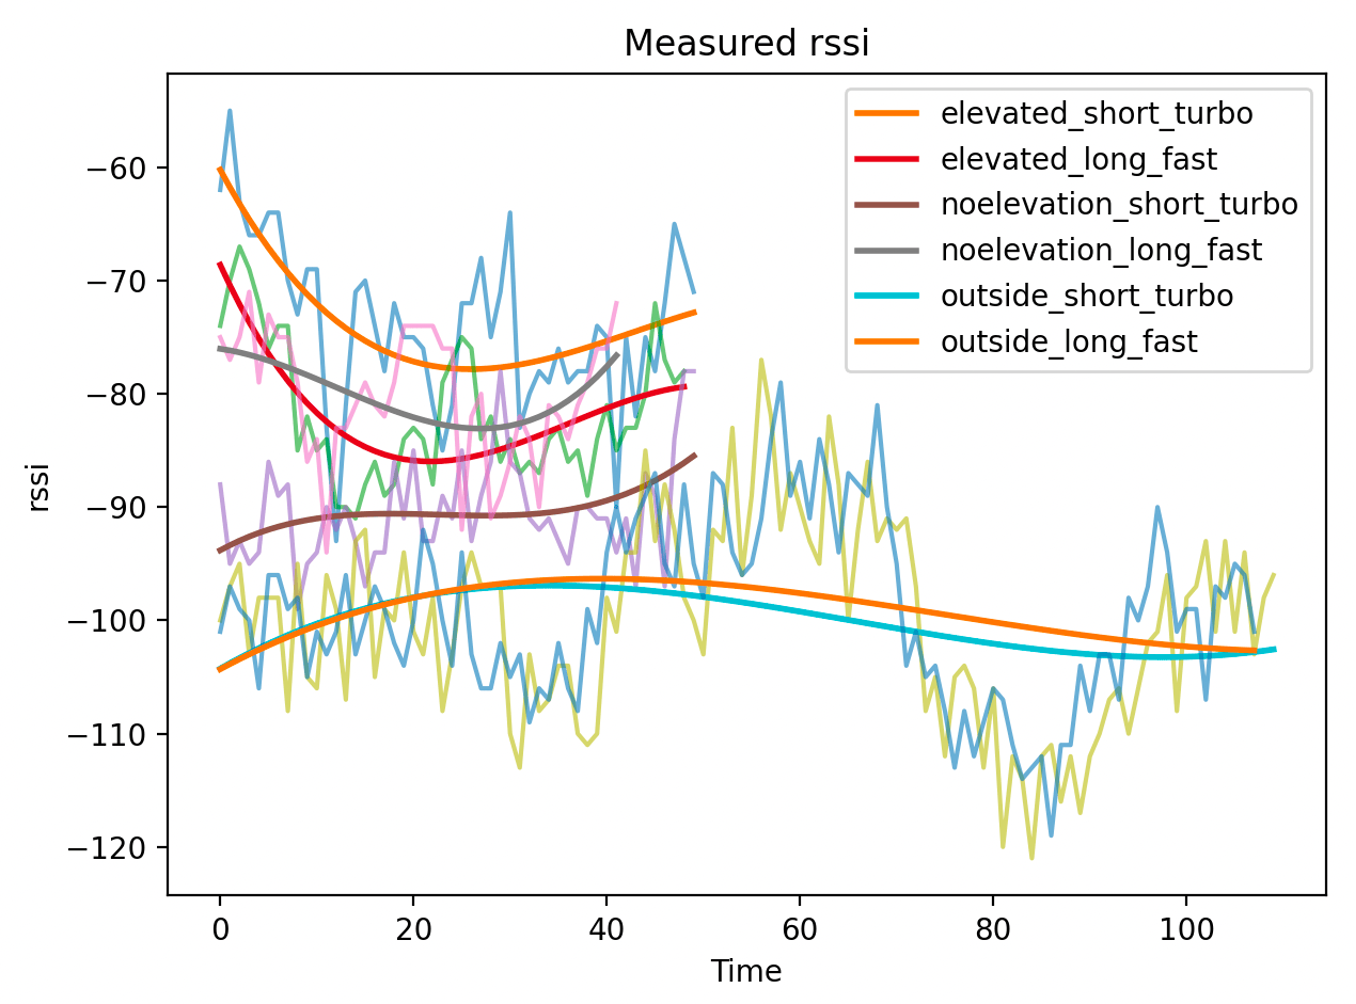
\includegraphics[width=0.7\linewidth]{images/image16.png}
    \caption{SMU Range Test RSSI Measurements}
    \label{fig:smu_rangetest_rssi}
\end{figure}

\begin{figure}[htbp]
    \centering
    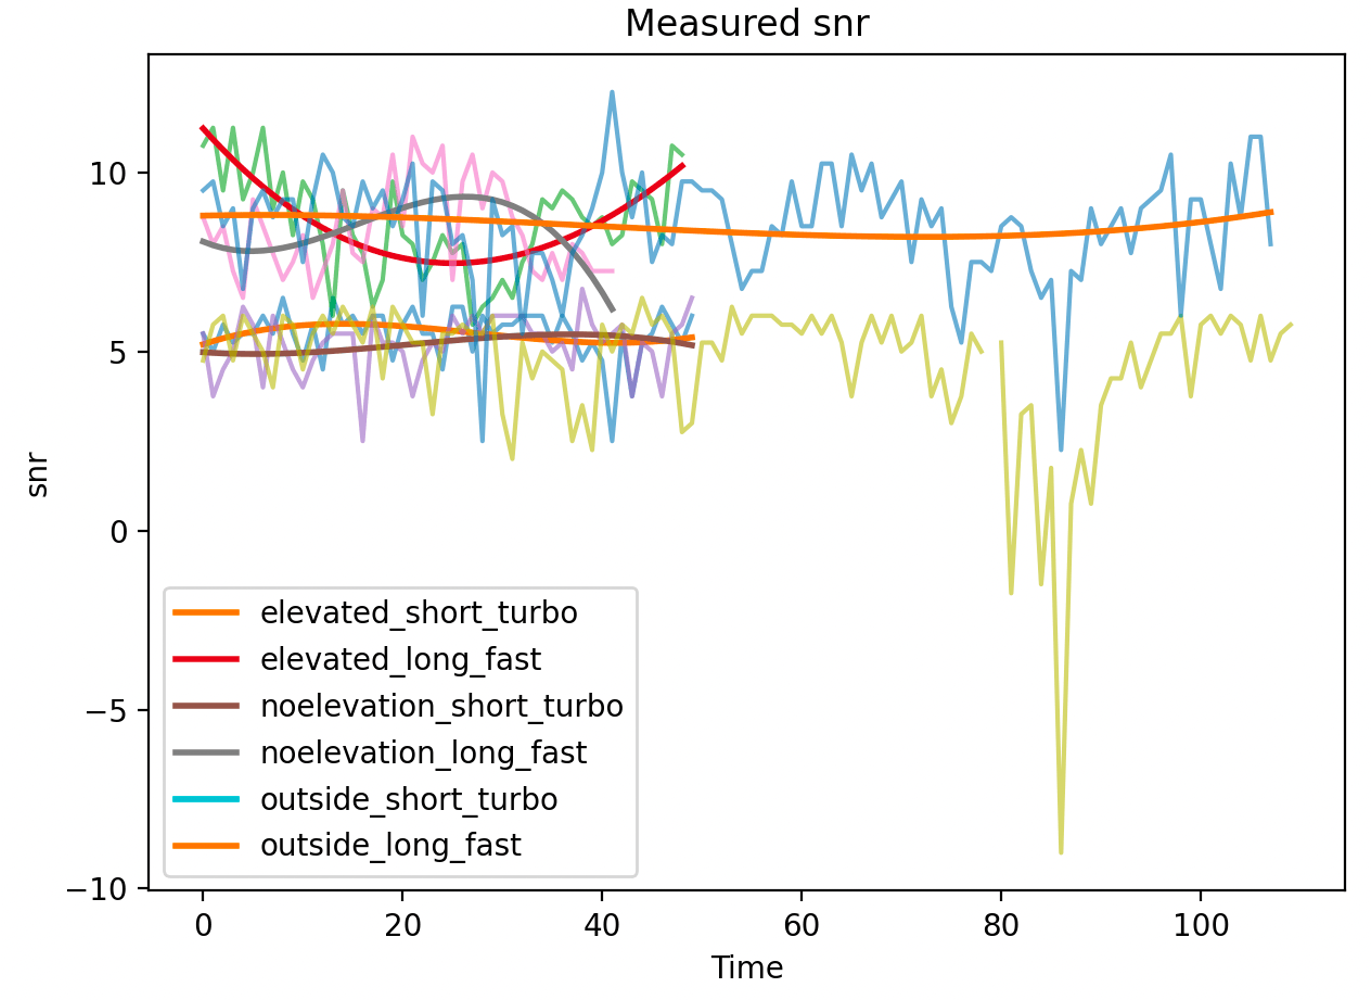
\includegraphics[width=0.7\linewidth]{images/image32.png}
    \caption{SMU Range Test SNR Measurements}
    \label{fig:smu_rangetest_snr}
\end{figure}

\begin{figure}[htbp]
    \centering
    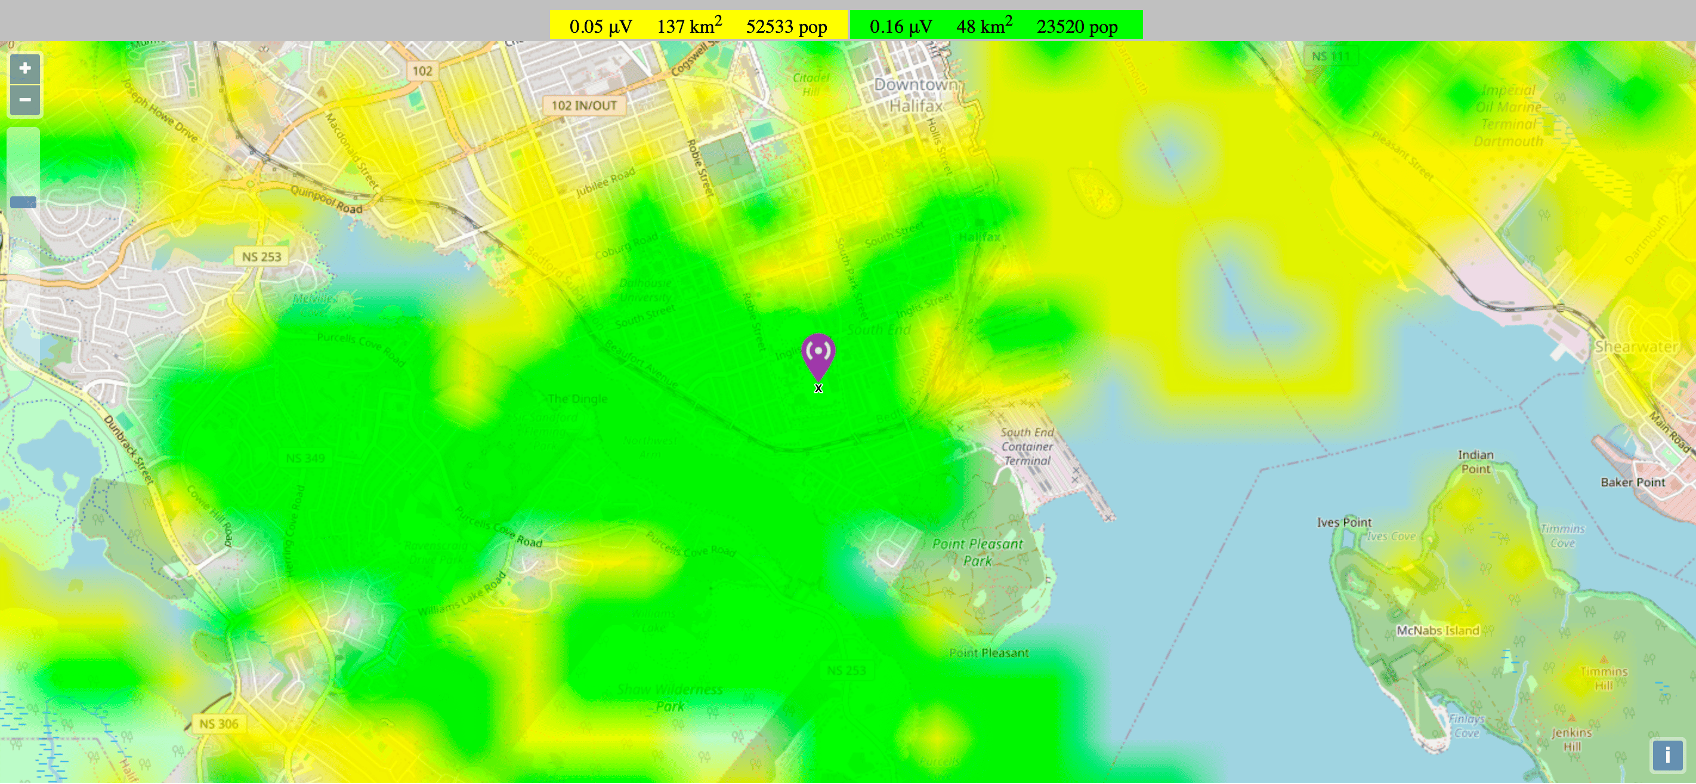
\includegraphics[width=0.7\linewidth]{images/image38.png}
    \caption{Radio Mobile Propagation Simulation}
    \label{fig:radiomobile}
\end{figure}

\begin{figure}[htbp]
    \centering
    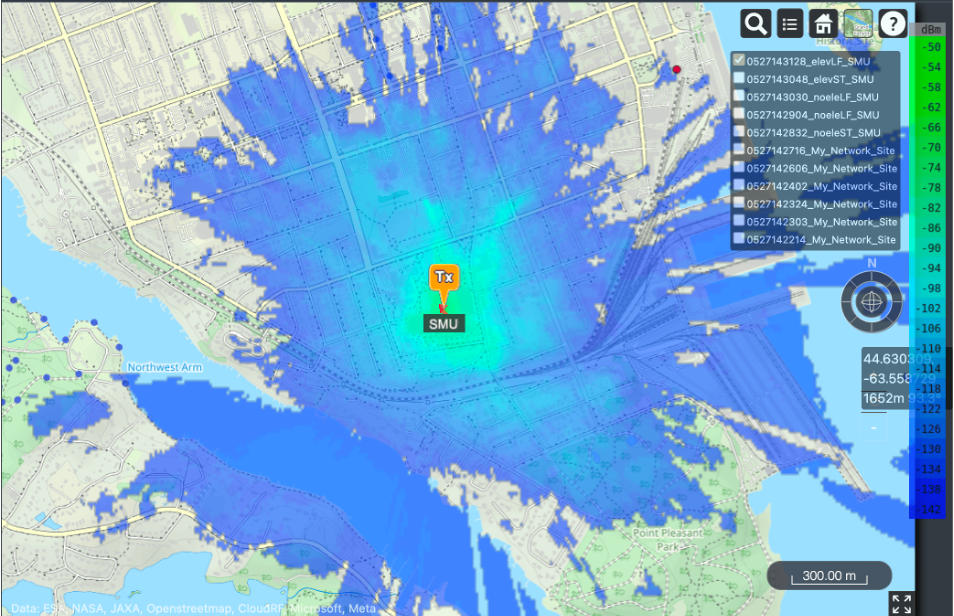
\includegraphics[width=0.7\linewidth]{images/image22.png}
    \caption{CloudRF Propagation Simulation}
    \label{fig:cloudrf}
\end{figure}

The data and results gathered through these tests could have been strengthened with GPS coordinates included in sent packets.

\FloatBarrier
\subsubsection{Bike Range Test}

The next range test was conducted in the Halifax area, with the mobile node attached to a bike. The goal of the test was to determine the general effective zero-hop range between two nodes. 

For each test, the receiving node was left stationary at the Goldberg Computer Science building, in room 211, while the other node was moving on a bike. Both nodes were connected by serial to a computer to automate the sending and storing of packet data through the Meshtastic Python interface. During each test, the node would be taken around various areas of Halifax and the Dalhousie campus, sending packets every 10 seconds. The Meshtastic node configuration was set to either LONG\_FAST or SHORT\_TURBO. Packet payloads contained the following variables: receivedTime, nodeID, RSSI, SNR, lat, long, alt and hopsUsed. The GPS function on the T-Beam did not work, so GPS data was obtained every 10 seconds from an iPhone, then sent to the sender computer via HTTP. 

The results show that the effective zero-hop range of two T-Beam running Meshtastic firmware on LONG\_FAST is approximately 500 meters. The connection can generally survive about one to two buildings or major obstructions, potentially more if there is a strong decrease in elevation to the receiving node. If both nodes are adjacent on a street, the street acts as a propagation corridor and extends its range significantly. Results show that down an adjacent street, nodes can reach as far as 1 kilometer, and potentially further. Even when the connection was lost as the signal strength fell below the sensitivity limit, the signal quality often stayed strong. If LoRa technology were used within a city for some use case, it would be beneficial to strategically place nodes down adjacent streets, in conjunction with other factors including elevation, line of sight and building density. Furthermore, it would have saved lots of time to use a pre-made Meshtastic range test module instead of building a range test system in Python from scratch.

\begin{figure}[htbp]
    \centering
    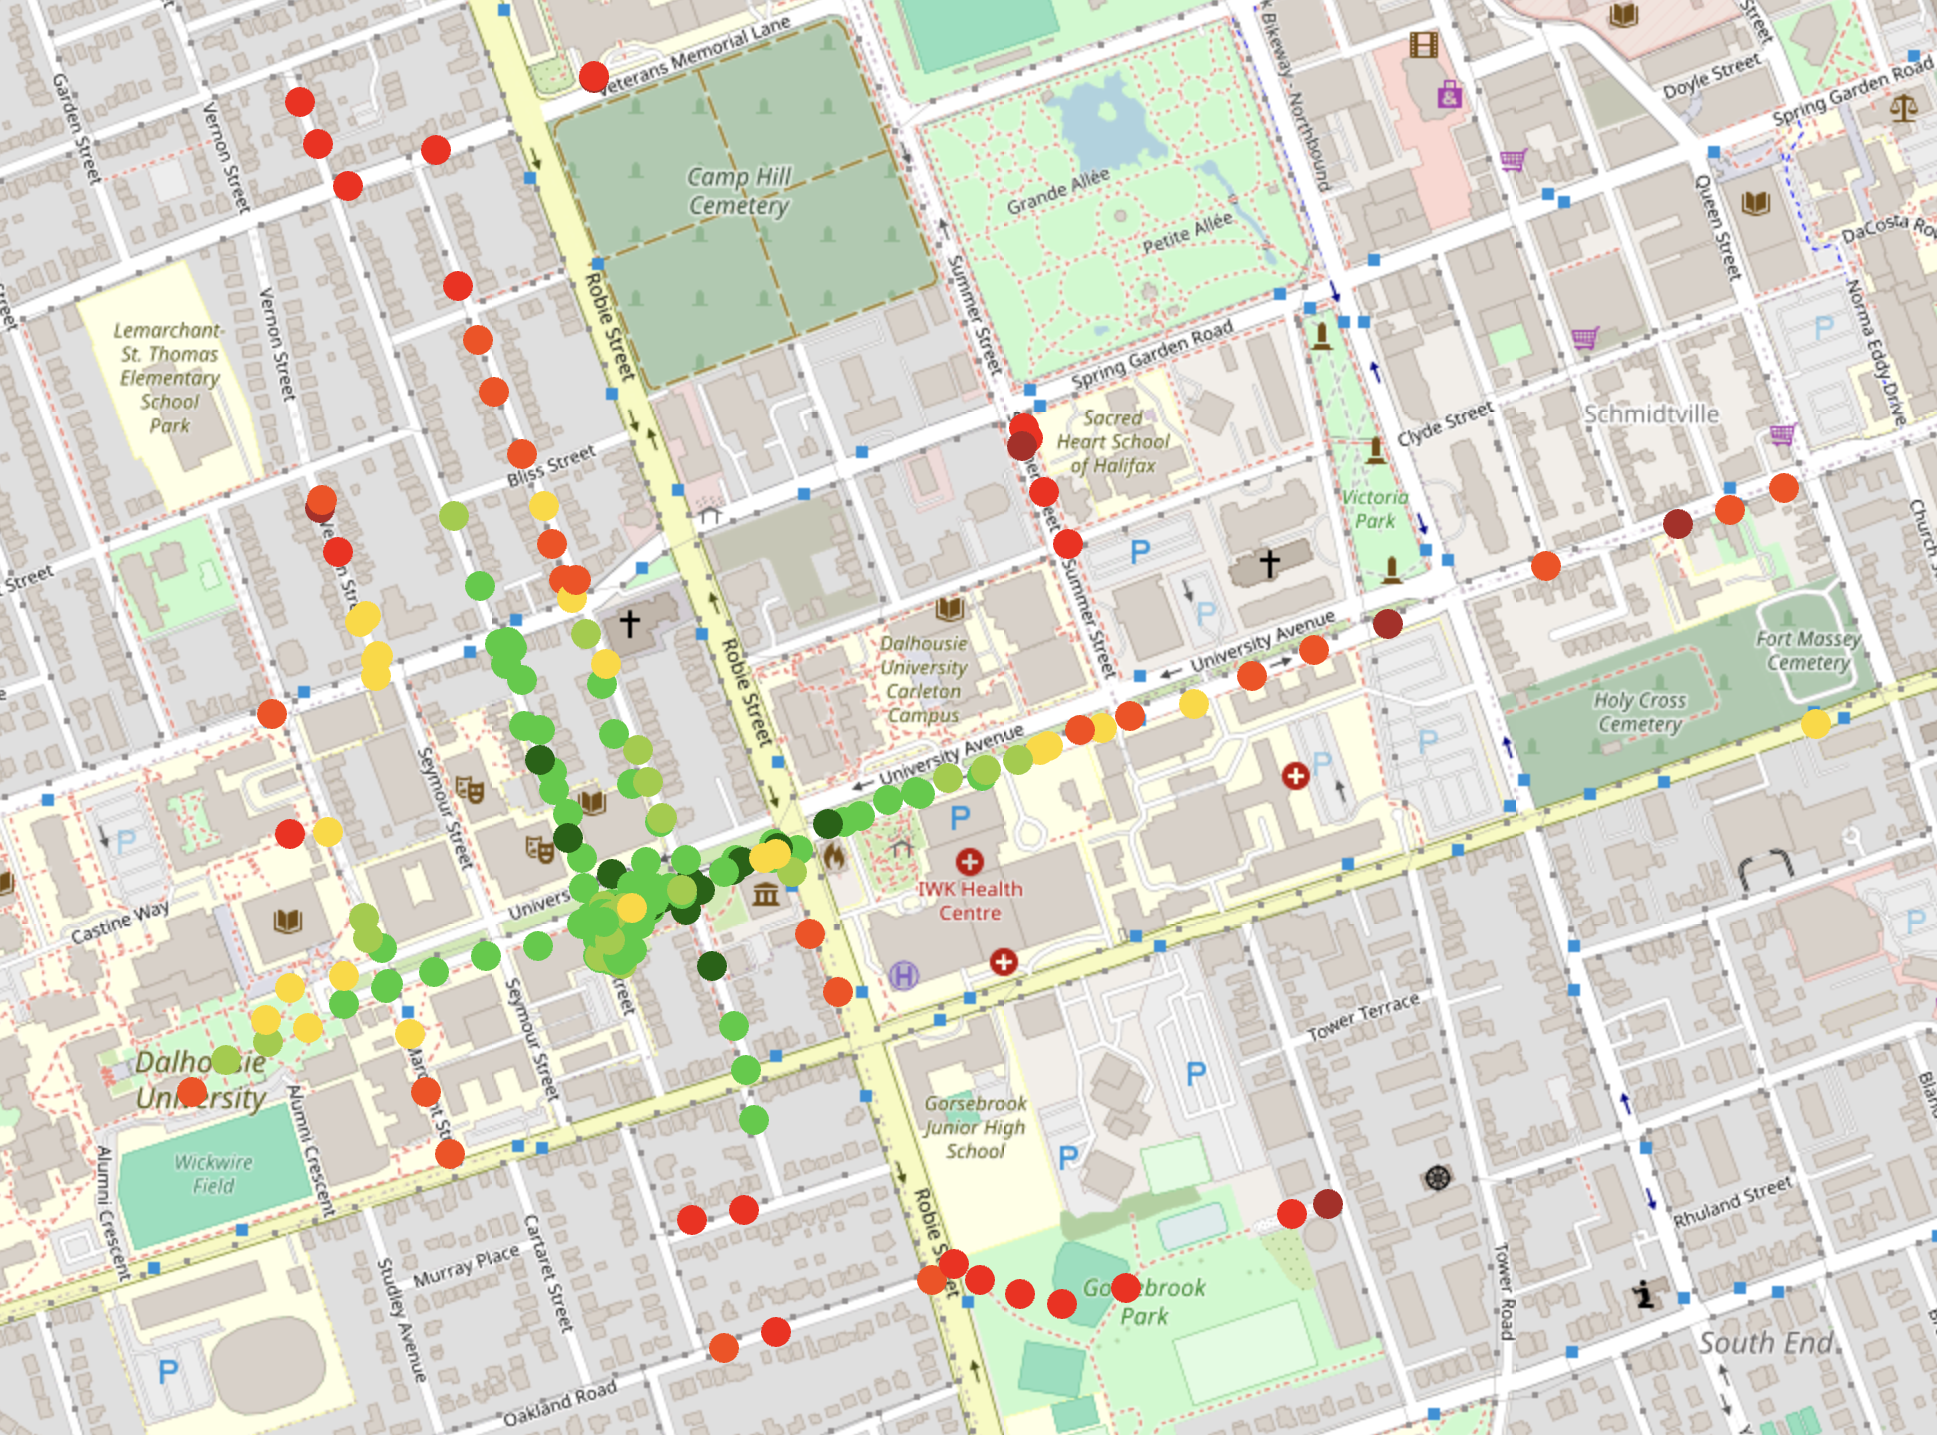
\includegraphics[width=0.7\linewidth]{images/image39.png}
    \caption{Bike Range Test SNR Values}

    \vspace{2mm}

    \begin{minipage}{\linewidth}
        \centering
        \small
        \textbf{Legend (SNR):}\\[2pt]
        10 dB = dark green\\
        5 to 10 dB = lime green\\
        0 to 5 dB = yellow-green \\
        $-5$ to 0 dB = gold\\
        $-10$ to $-5$ dB = orange-red\\
        $-15$ to $-10$ dB = red \\
        $-20$ to $-15$ dB = firebrick\\
        $\leq -20$ dB = dark red
    \end{minipage}
    
    \label{fig:bike_test_snr}
\end{figure}

\begin{figure}[htbp]
    \centering
    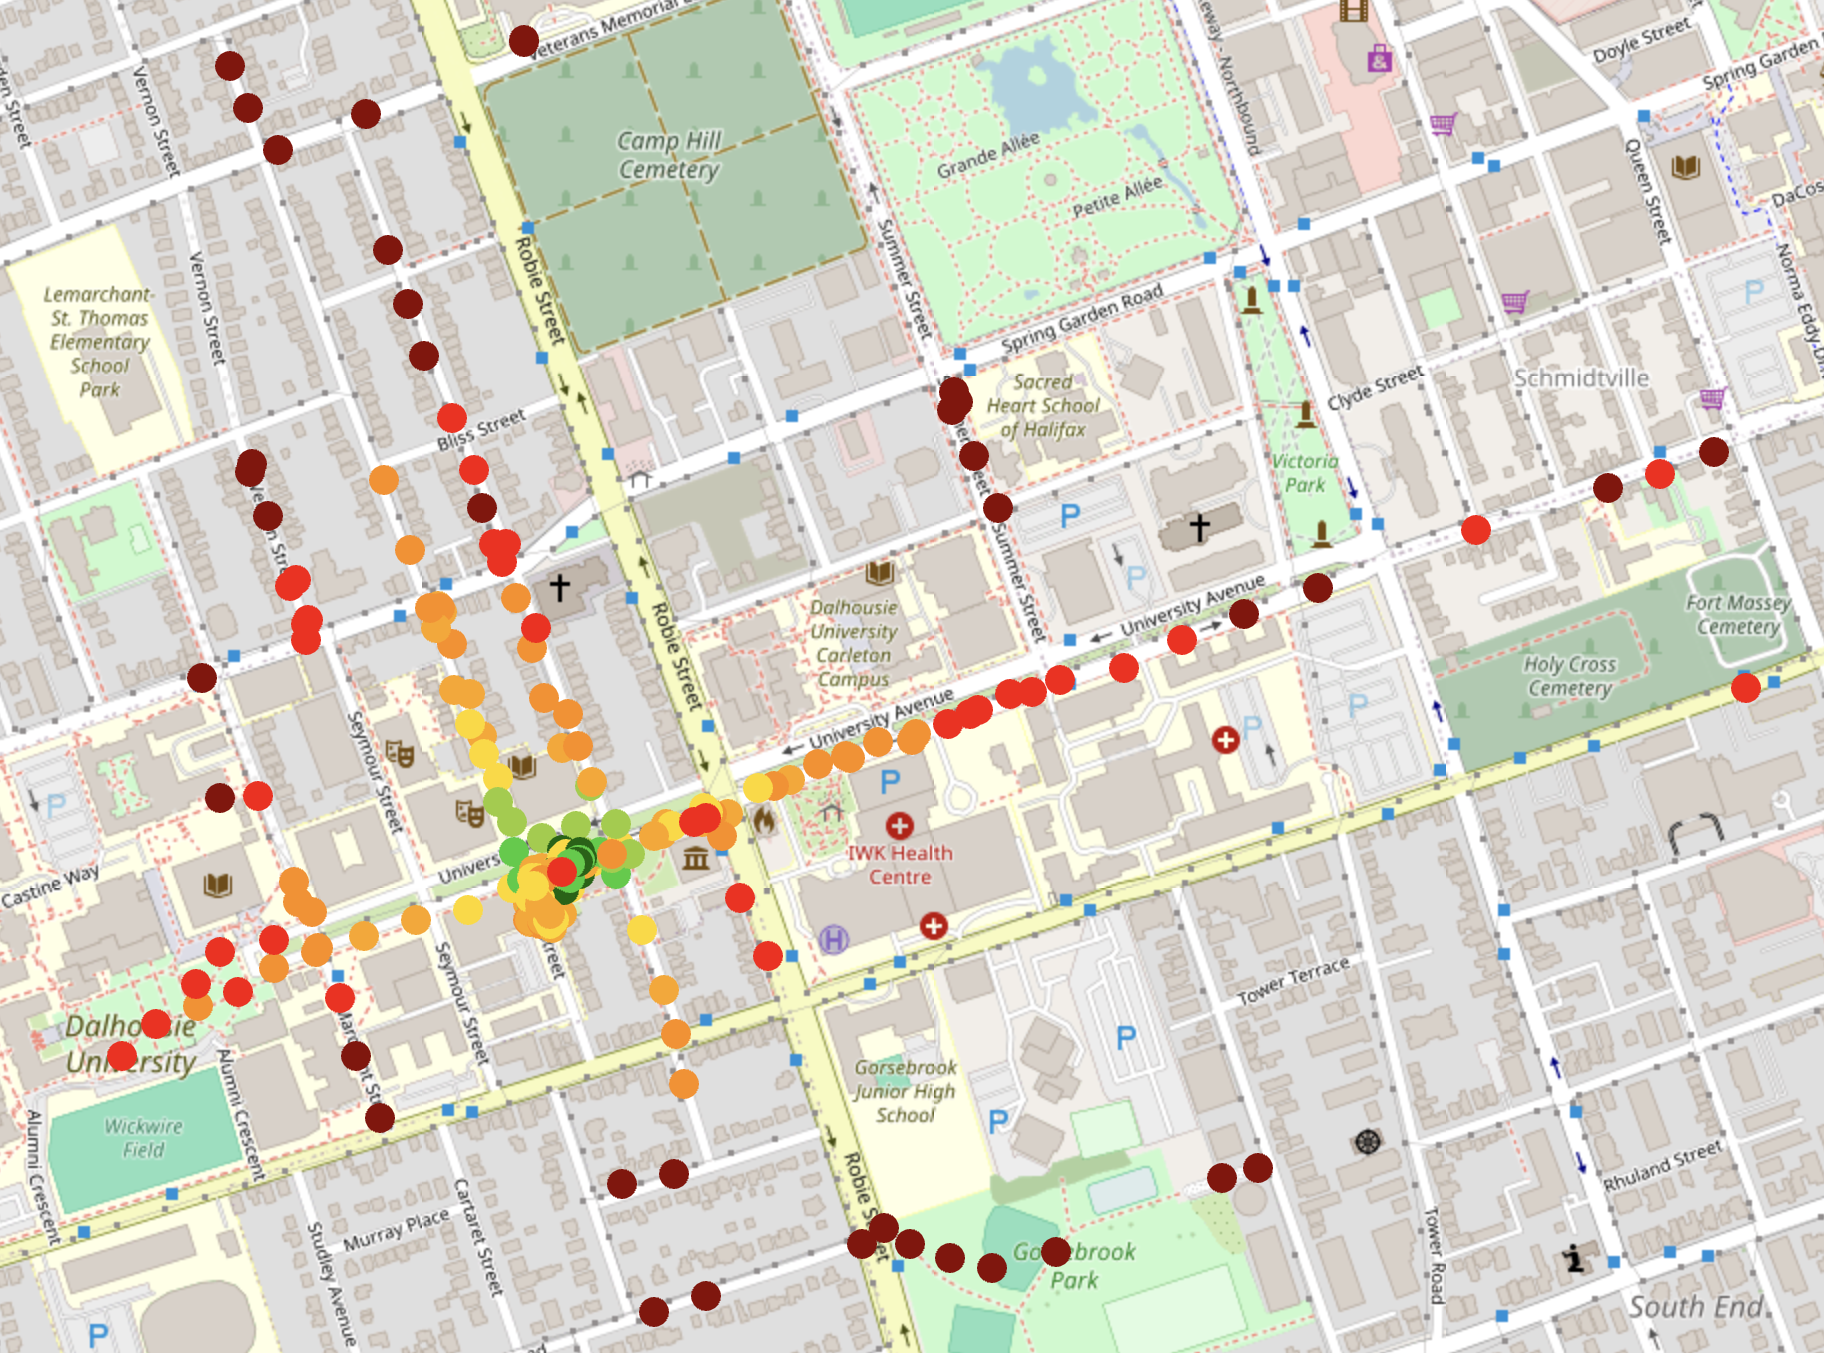
\includegraphics[width=0.7\linewidth]{images/image35.png}
    \caption{Bike Range Test RSSI Values}

    \vspace{2mm}

    \begin{minipage}{\linewidth}
        \centering
        \small
        \textbf{Legend (RSSI):}\\[2pt]
        $-70$ dBm = dark green\\
        $-80$ to $-70$ dBm = lime green\\
        $-90$ to $-80$ dBm = green \\
        $-100$ to $-90$ dBm = gold\\
        $-110$ to $-100$ dBm = orange\\
        $-120$ to $-110$ dBm = dark orange \\
        $-130$ to $-120$ dBm = red\\
        $\leq -130$ dBm = dark red
    \end{minipage}
    
    \label{fig:bike_test_rssi}
\end{figure}

\FloatBarrier
\subsubsection{Bike Comparison Test}
This test was a shorter repeat of the bike range test (Figures~\ref{fig:bike_test_snr} and~\ref{fig:bike_test_rssi}), except with two different firmware systems. The goal of this test was to determine if there were any major underlying differences in performance between Meshtastic and MeshCore, even when all of the configuration settings were the same. This was to make sure that for future tests using MeshCore, identical configuration settings could be treated as equivalent to those in Meshtastic. In the early stages of the internship, it was believed that MeshCore would play a large role. However, this was not the case as MeshCore was not used in any future tests.

There were very few differences in settings and methods for this test compared to the previous range test. The one major difference was that the sender node was not a T-Beam but a LILYGO LoRa32 v1.6.1 radio. This device has the same SX1276 chip, but came with a much shorter default antenna, likely with lower gain. All of the configuration settings in Table~\ref{tab:comparison_test_settings} were applied to both firmware versions:

\begin{table}[htbp]
    \centering
    \caption{LoRa Settings for Comparison Test}
    \label{tab:comparison_test_settings}
    \begin{tabularx}{\textwidth}{lX}
        \toprule
        \textbf{Setting} & \textbf{Value} \\
        \midrule
        Frequency & 906.875 MHz \\
        Bandwidth & 250 kHz \\
        Spreading Factor & 11 \\
        Coding Rate & 4/5 \\
        Transmit Power & 20 dBm \\
        \bottomrule
    \end{tabularx}
\end{table}

The results were as expected: both firmware performed similarly under identical configuration settings. The range of the sender node down University Avenue in this test was much shorter than on the previous range test. This is likely because the sender node used the smaller antenna on the LoRa32. This test demonstrates that, for zero-hop communication, Meshtastic and MeshCore perform equally under the same LoRa settings.

\begin{figure}[htbp]
    \centering
    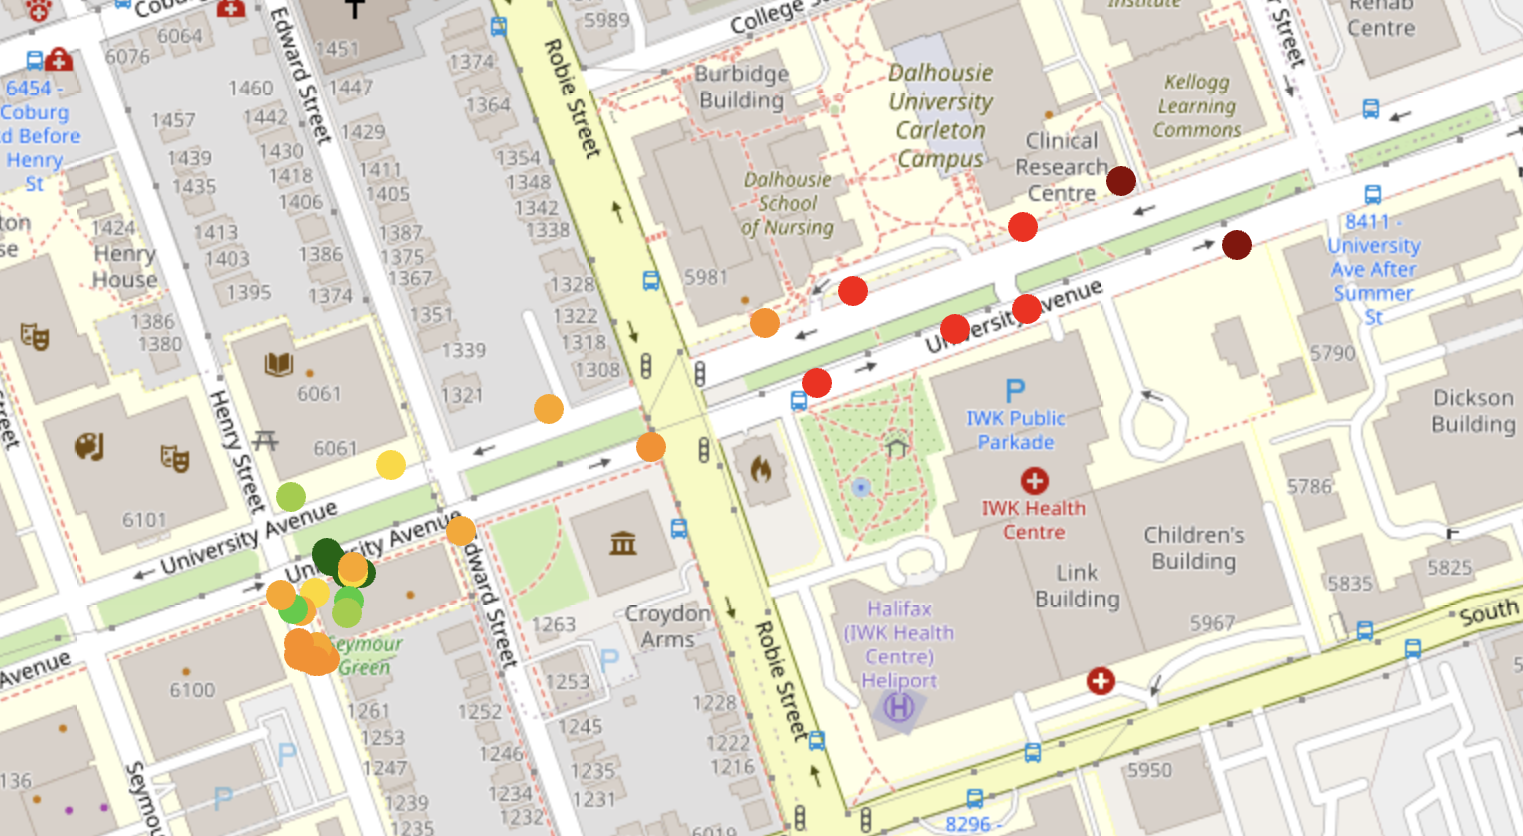
\includegraphics[width=0.7\linewidth]{images/image17.png}
    \caption{Firmware Comparison Test Meshtastic RSSI Measurements}
    \label{fig:comp_test_mt_rssi}
\end{figure}

\begin{figure}[htbp]
    \centering
    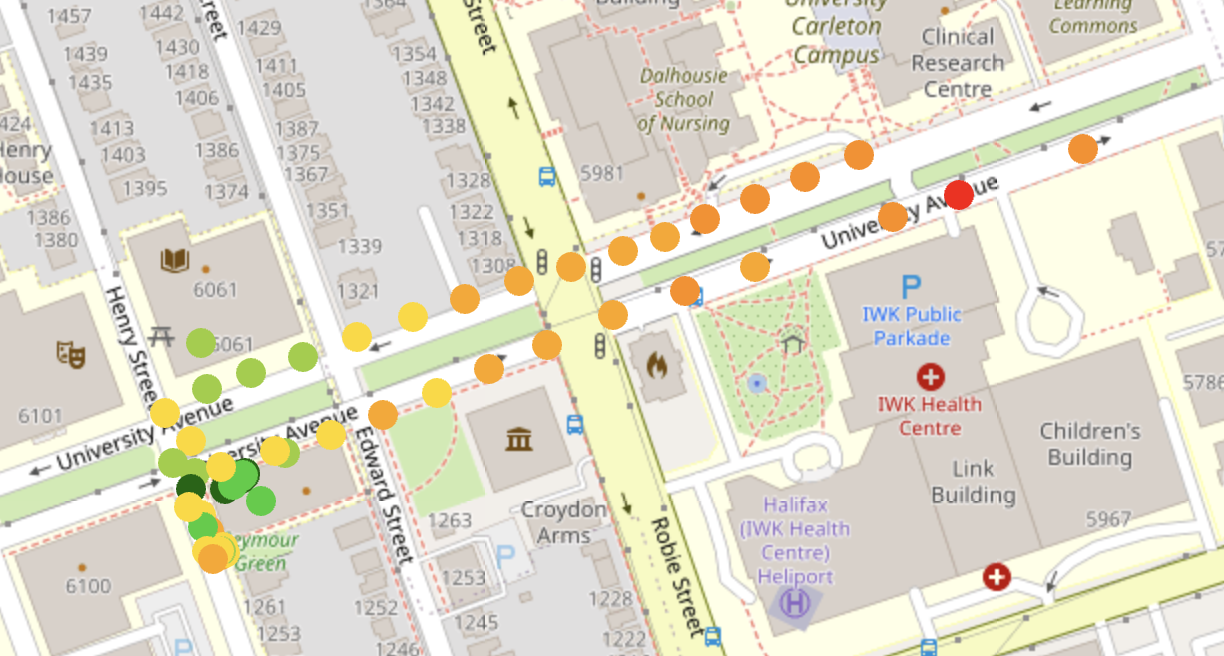
\includegraphics[width=0.7\linewidth]{images/image8.png}
    \caption{Firmware Comparison Test MeshCore RSSI Measurements}
    \label{fig:comp_test_mc_rssi}
\end{figure}

\begin{figure}[htbp]
    \centering
    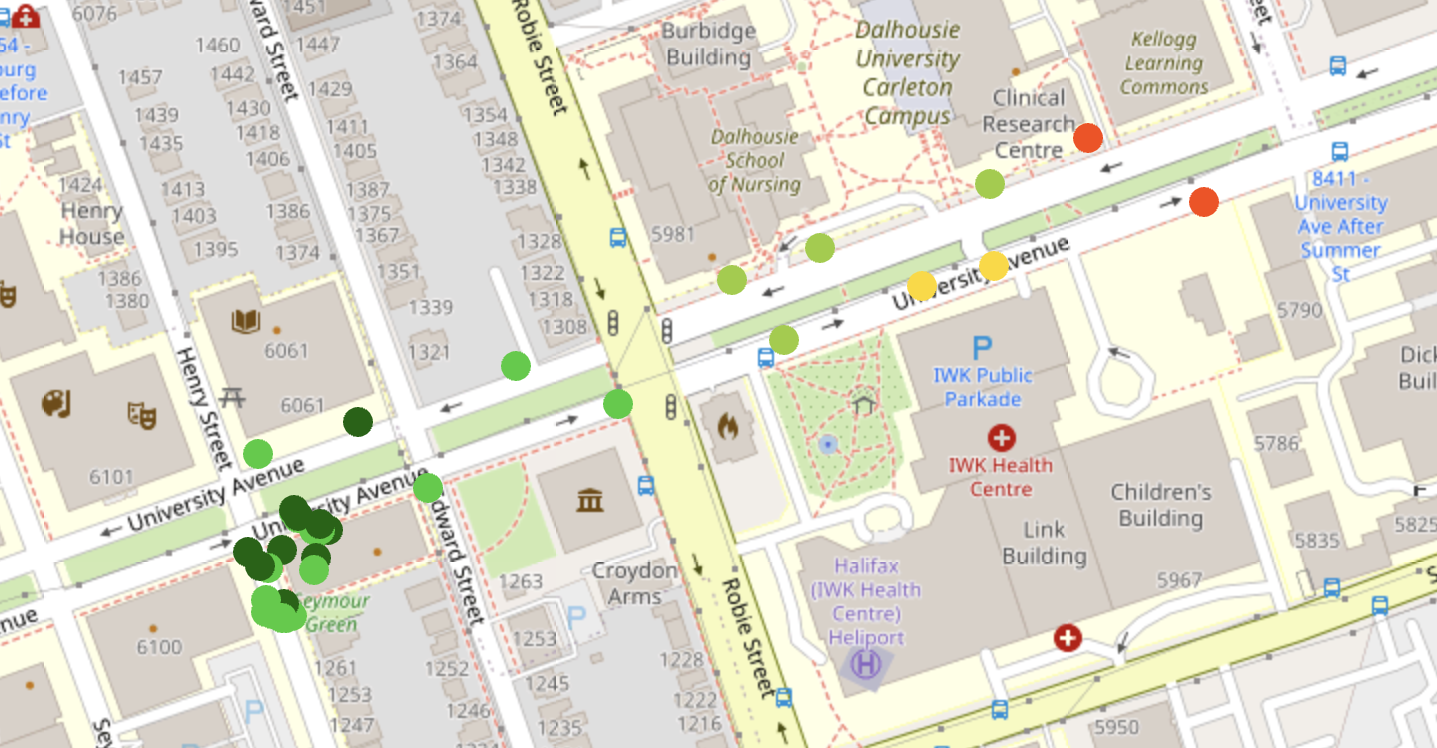
\includegraphics[width=0.7\linewidth]{images/image7.png}
    \caption{Firmware Comparison Test Meshtastic SNR Measurements}
    \label{fig:comp_test_mt_snr}
\end{figure}

\begin{figure}[htbp]
    \centering
    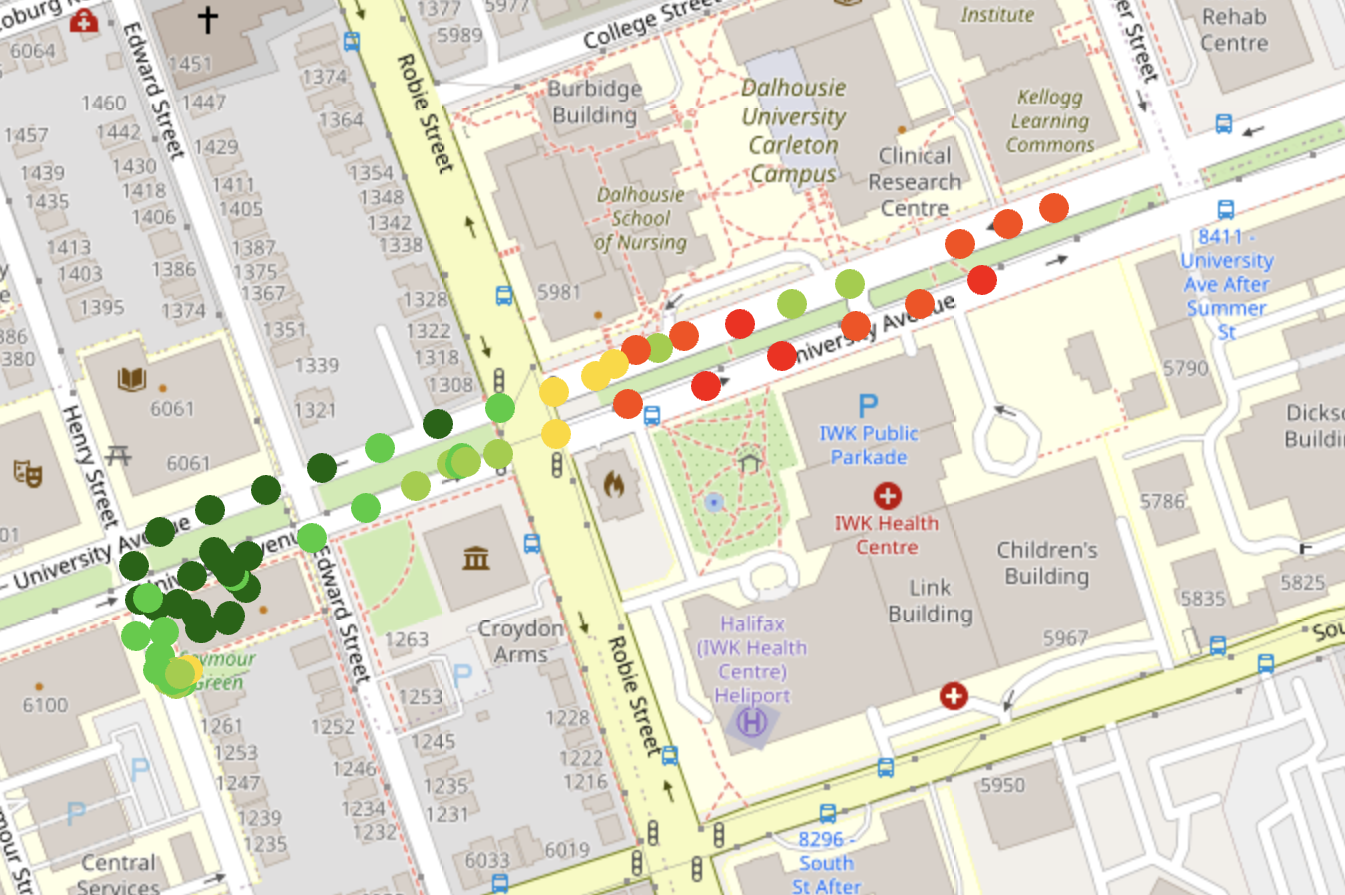
\includegraphics[width=0.7\linewidth]{images/image37.png}
    \caption{Firmware Comparison Test MeshCore SNR Measurements}
    \label{fig:comp_test_mc_snr}
\end{figure}

\FloatBarrier
\subsection{Dalhousie Meshtastic Campus Deployment Tests}

After conducting baseline tests for zero-hop performance of LoRa mesh devices, a testbed was required to begin conducting tests in which nodes needed multiple hops to communicate. Thus, six nodes were strategically placed around Dalhousie campus. 

The first iteration of the testbed was a success. Devices were placed at the following locations: Goldberg 211, Life Sciences Center (LSC) Biology Wing 8th floor study area, Collaborative Health Education Building 2nd floor study area (CHEB), Dalplex 2nd floor (near studios), SUB 2nd floor conference room and McCain Arts Building room 2130. Nodes were eventually moved to other locations, including Rowe 5001 and James Dunn 221C. A second node was eventually added to the Goldberg Playground 235 and connected to a desktop computer for monitoring purposes. The only problematic node was the node at the CHEB. Even though the node was placed next to a window on University Avenue, which is adjacent to the Computer Science Building, it still could not connect to the rest of the mesh often enough. This node was eventually moved elsewhere. Furthermore, the node placed at the Dalplex was taken by the Dalplex staff and given to security. The node could not be placed back at the Dalplex without permission, and it was decided before negotiations that it would simply be best to leave the node elsewhere. This change was made after many tests were already conducted.

\begin{figure}[htbp]
    \centering
    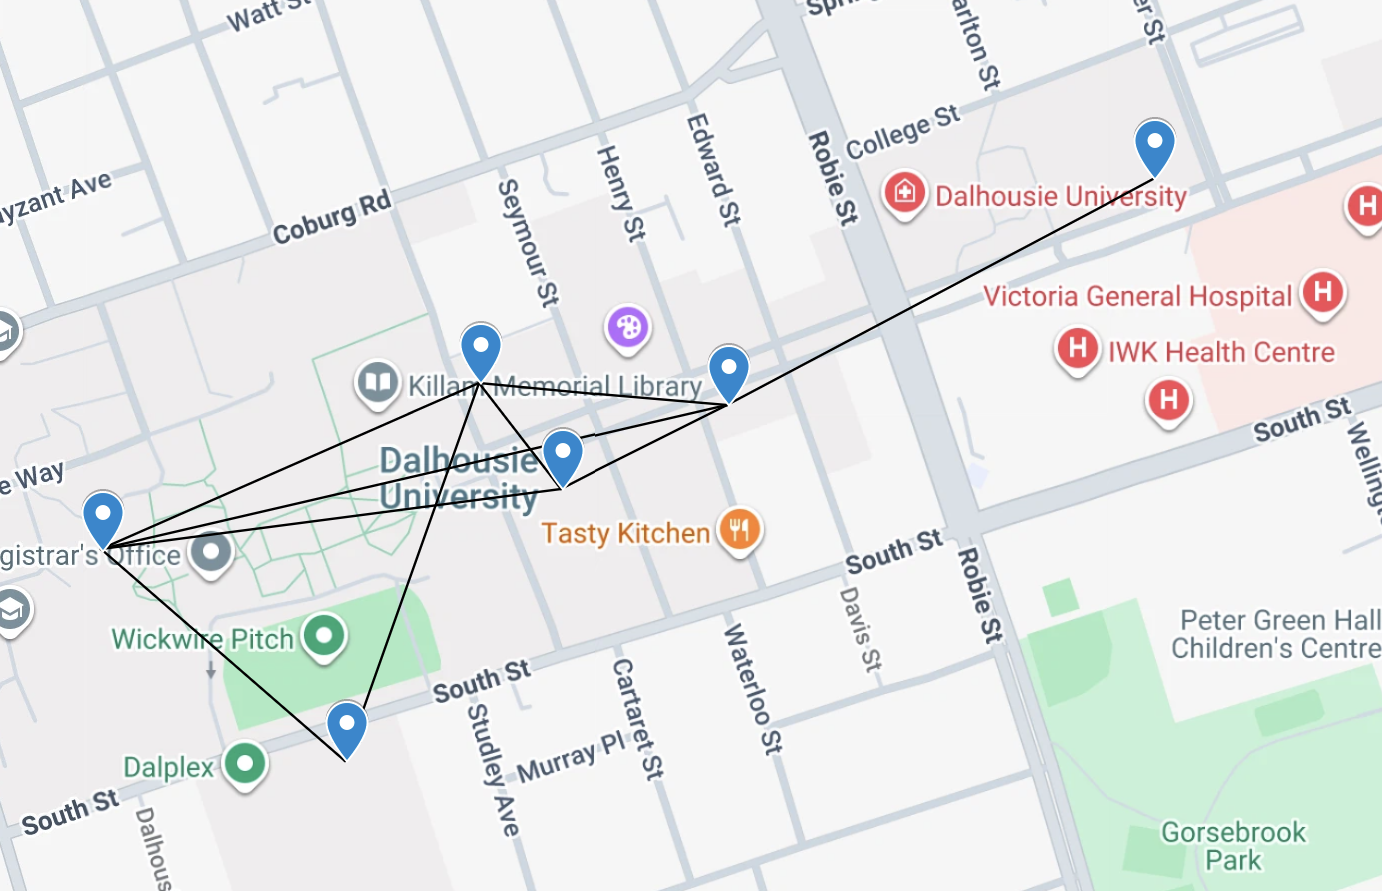
\includegraphics[width=0.7\linewidth]{images/image11.png}
    \caption{First Iteration of the Campus Deployment}
    \label{fig:first_campus_deployment}
\end{figure}

\begin{figure}[htbp]
    \centering
    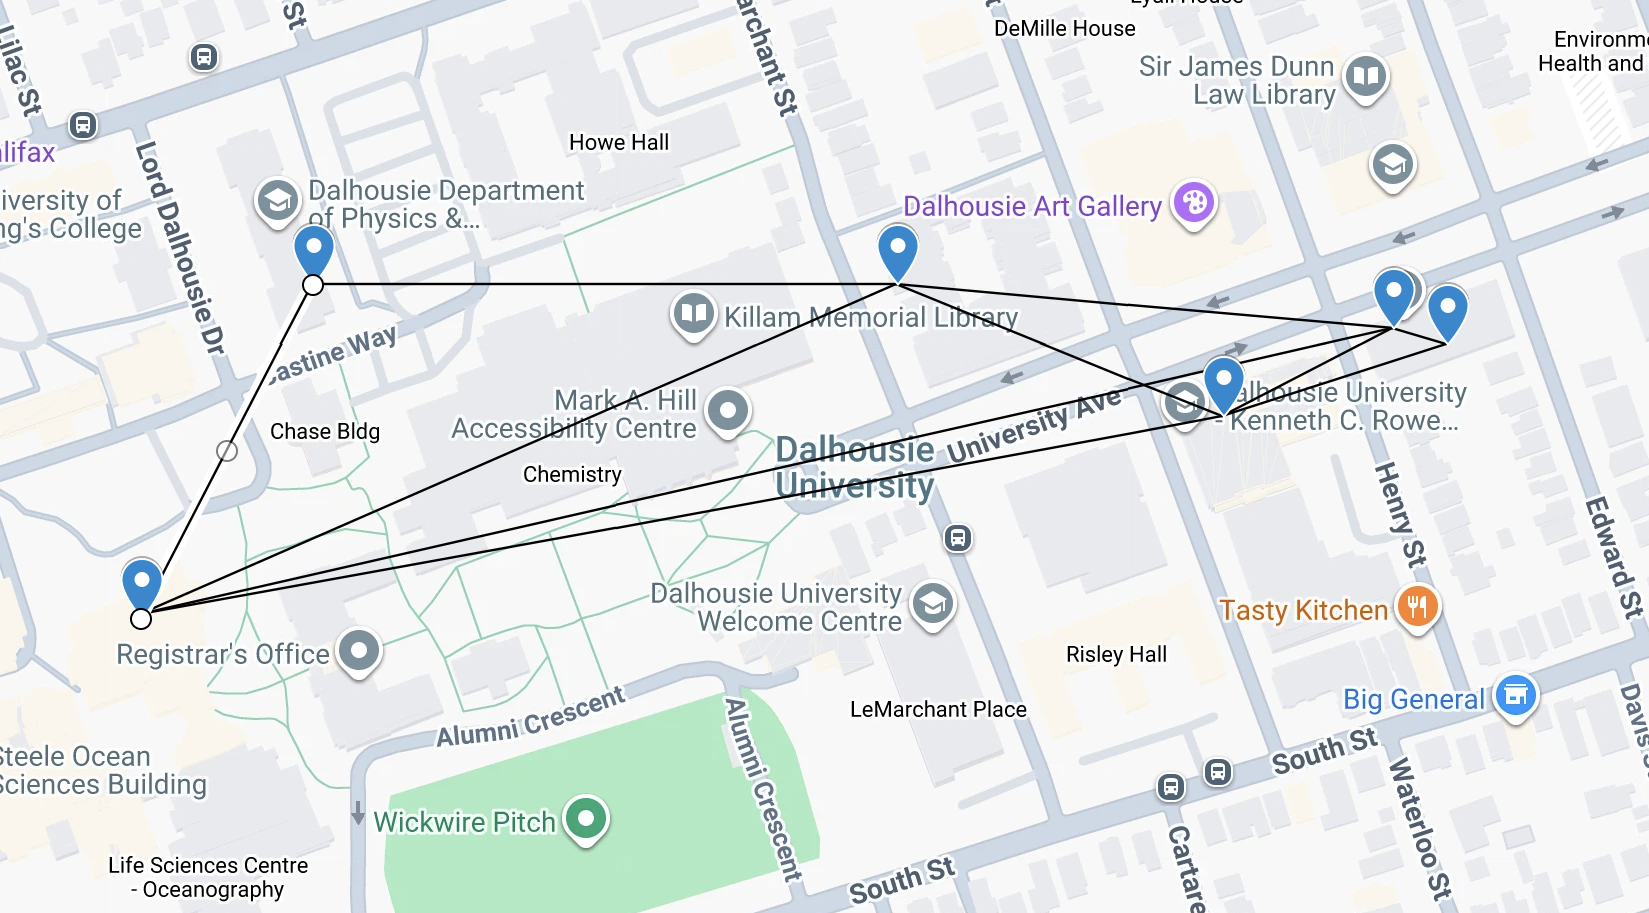
\includegraphics[width=0.7\linewidth]{images/image33.png}
    \caption{Final Iteration of the Campus Deployment}
    \label{fig:final_campus_deployment}
\end{figure}

\begin{table}[htbp]
    \centering
    \caption{All Node Locations in Campus Deployment}
    \label{tab:node_locations}
    \begin{tabularx}{\textwidth}{X l X l}
        \toprule
        \textbf{Name} & \textbf{Node ID} & \textbf{Room} & \textbf{Hardware }\\
        \midrule
        Goldberg Window Node & !ea2468b0 & Room 211 & LILYGO T-Beam\\
        Goldberg Desktop Node & !6c73daa0 & Playground 235 & LILYGO LoRa32\\
        Rowe Business Building Node & !dadfb0cc & Room 5001 & LILYGO T-Beam\\
        LSC Biology Node & !dadfb008 & 8th floor study area & LILYGO T-Beam\\
        McCain Arts Building Node & !dadfb6c8 & Room 2130 & LILYGO T-Beam\\
        Dalplex Node & !dadfb8d4 & 2nd floor studios hallway & LILYGO T-Beam\\
        Collaborative Health Education Building Node & !dadfb03c & 2nd floor study area & LILYGO T-Beam\\
        James Dunn Building Node & !dadfb03c & Room 221C & LILYGO T-Beam\\
        \bottomrule
    \end{tabularx}
\end{table}

\FloatBarrier
\subsubsection{Single-Route Multi-Hop Message Testing}

The first test using the campus testbed was a baseline test where packets were sent between two nodes at a distance at which multiple hops needed to be used. The goal of the test was to examine how performance changes as hops are added to the route and to determine at what point a small mesh becomes congested.

The Goldberg node would send 50 packets at varying intervals to the Dalplex node, while simultaneously waiting for an ACK and recording information contained in the ACK. The receiving node would listen for packets, send ACKs when packets were received and record the data in a CSV file. Both of these workflows were conducted using the Meshtastic Python CLI to automate the sending and recording of packet data. The intervals at which messages were sent included 5 seconds, 20 seconds, 40 seconds and 1 minute. For each interval, multiple tests were conducted, each at two different times of day: morning and afternoon. Morning is classified as anything from 8 a.m. to 1 p.m., while afternoon is anytime from 1 p.m. to 6 p.m. 

All of the devices in the campus mesh were T-Beam. Furthermore, all devices were flashed with default Meshtastic firmware using the LONG\_FAST LoRa preset. Packet payloads included several metrics, including packet ID, receiver node ID, sender node ID, final byte of the address of the most recent hop, delivery rate, latency (end-to-end), RSSI and SNR. To make the latency calculations as accurate as possible, both nodes were synchronized to the same NTP server before any scripts began running. Latency measurements are unidirectional and thus do not account for how long it takes for the ACK to be received.

\begin{figure}[htbp]
    \centering
    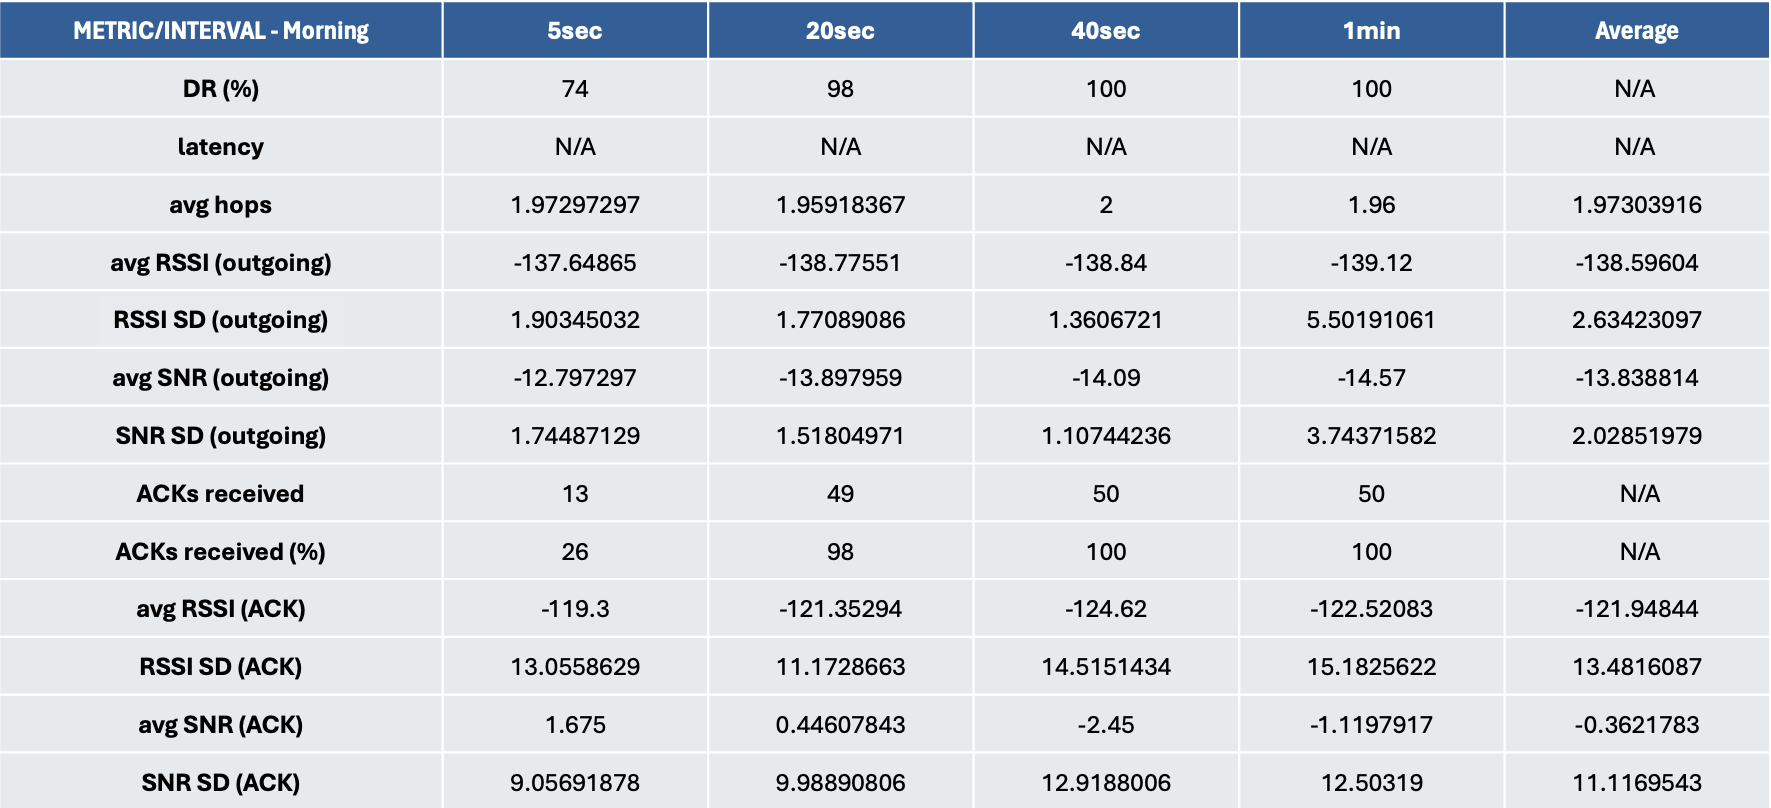
\includegraphics[width=0.7\linewidth]{images/image13.png}
    \caption{Single-Route Multi-Hop Morning Test Results}
    \label{fig:morning_results}
\end{figure}

\begin{figure}[htbp]
    \centering
    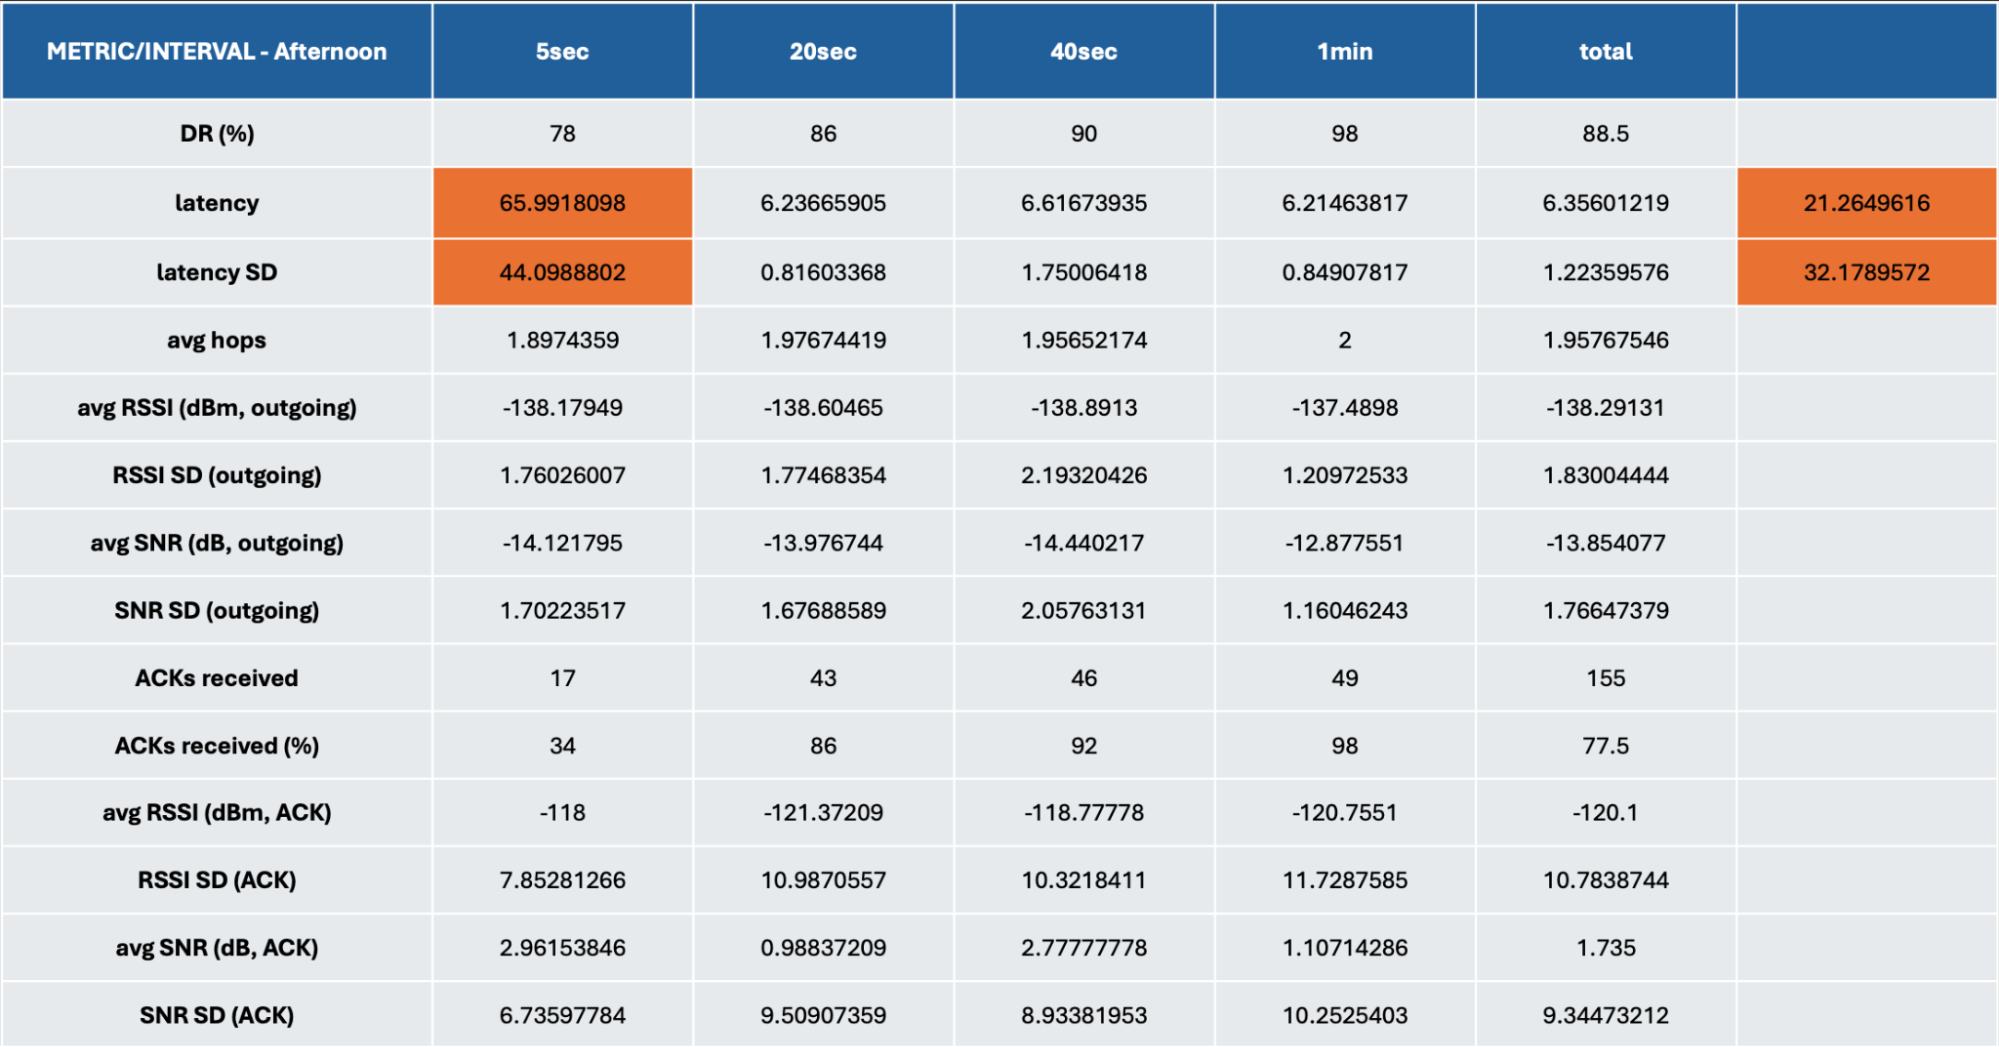
\includegraphics[width=0.7\linewidth]{images/image9.png}
    \caption{Single-Route Multi-Hop Afternoon Test Results}
    \label{fig:afternoon_results}
\end{figure}

\begin{figure}[htbp]
    \centering
    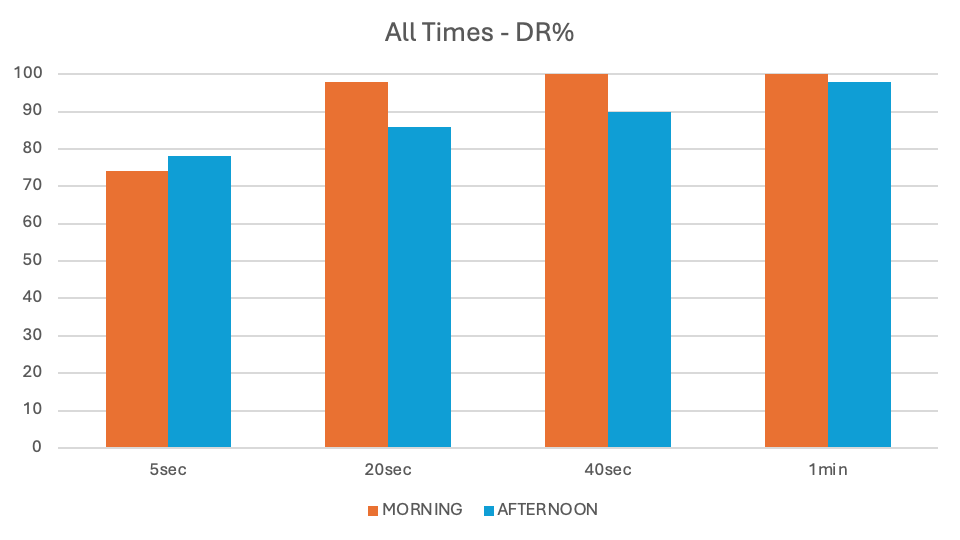
\includegraphics[width=0.7\linewidth]{images/image14.png}
    \caption{Single-Route Multi-Hop Delivery Rate Results}
    \label{fig:dr_plex_to_gb}
\end{figure}

\begin{figure}[htbp]
    \centering
    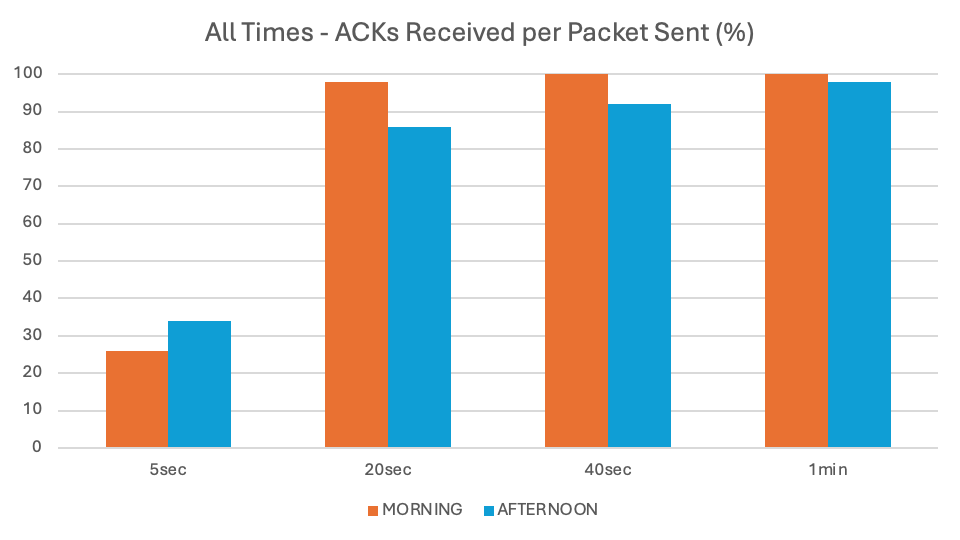
\includegraphics[width=0.7\linewidth]{images/image26.png}
    \caption{Single-Route Multi-Hop ACK Reception Rate Results}
    \label{fig:ack_rate_plex_to_gb}
\end{figure}

In Meshtastic, a message is considered successful and is shown on the user interface if both the message and the ACK are received. Thus, it is important to make the distinction between the packet delivery rate and ACK delivery rate. Evidently, sending messages at a five-second interval causes too many collisions, thus resulting in very low ACK reception rates of 26\% and 34\%, in the morning and afternoon tests, respectively. Other intervals show similar ACK reception rates, thus indicating that the threshold at which messages can be sent between two nodes is somewhere between 5 and 20 second sending intervals, below which messages begin colliding. For a route with 2 hops, it seems to take just about 6.2 seconds to reach the destination. Dividing the time to reach the destination by the number of hops plus one provides an estimate of, on average, how long it should take for one hop. Because the average number of hops used was 2, the average time to complete one hop is approximately 2 seconds. For communication where time is a serious constraint, it is important to limit the amount of potential hops as it can significantly impact speed.

\begin{equation}
    t_{\text{hop}} 
    = 
    \frac{t_{\text{destination}}}{N_\text{hops} + 1} 
    = 
    \frac{6.2}{2+1} 
    \approx 2.07
\end{equation}

The initial test plan had two routes being tested: Goldberg to Dalplex and LSC to CHEB. Tests between the LSC and CHEB were unsuccessful as the connection from the CHEB to any of the other nodes was not strong enough to consistently send messages. Thus, the focus became solely on tests from the Dalplex to the Goldberg. Additionally, the first tests had only two intervals: five seconds and one minute. However, more tests were conducted, and more intervals were introduced. Latency measurements are unidirectional and thus do not account for how long it takes for the ACK to be received. Timestamps were not added to the packets for the morning tests; thus, the latency measurements are only from the afternoon tests.

\FloatBarrier
\subsubsection{Dynamic Node Testing}

After gathering metrics on one stable, stationary path, it was only natural to begin collecting data under dynamic conditions including how Meshtastic reacts to change, how the managed flooding protocol adapts to a moving node and how this affects messaging performance. 

Similar to the previous range tests, there was a mobile sender node and a stationary receiver node. However, in this test, the sender node was moving at walking pace, and the campus testbed was used to force hops between nodes to observe routing changes. Packets were sent at the shortest allowed interval for traceroute packets to be sent: every 30 seconds. Packet data included delivery rate, sender ID, receiver ID, end-to-end latency, RSSI, SNR, geographic data and hops used. 

Like other tests, packet information was automated and captured using the Meshtastic Python CLI and devices were set to the default Meshtastic LONG\_FAST radio setting. The only configuration setting which was changed from the defaults was the sender node’s hop limit, which was changed from 3 to 7.

The delivery rate for packets sent on this route was 78\%, and the average latency was 6.44 seconds. Furthermore, the average hop latency was 2.62 seconds, which supports the previous claim that per-hop latency is about 2 seconds. The test results also show that the number of hops and latency in seconds have a strong linear relationship. The average latency when the number of hops changed was 8.70 seconds, while the average latency when the number of hops remained the same was 5.53 seconds. This is a 57.3\% increase in latency when there is a change in routing. A 78\% delivery rate shows that the managed flooding protocol is indeed resilient to moving nodes. However, it comes at the cost of a significant increase in latency.

\begin{figure}[htbp]
    \centering
    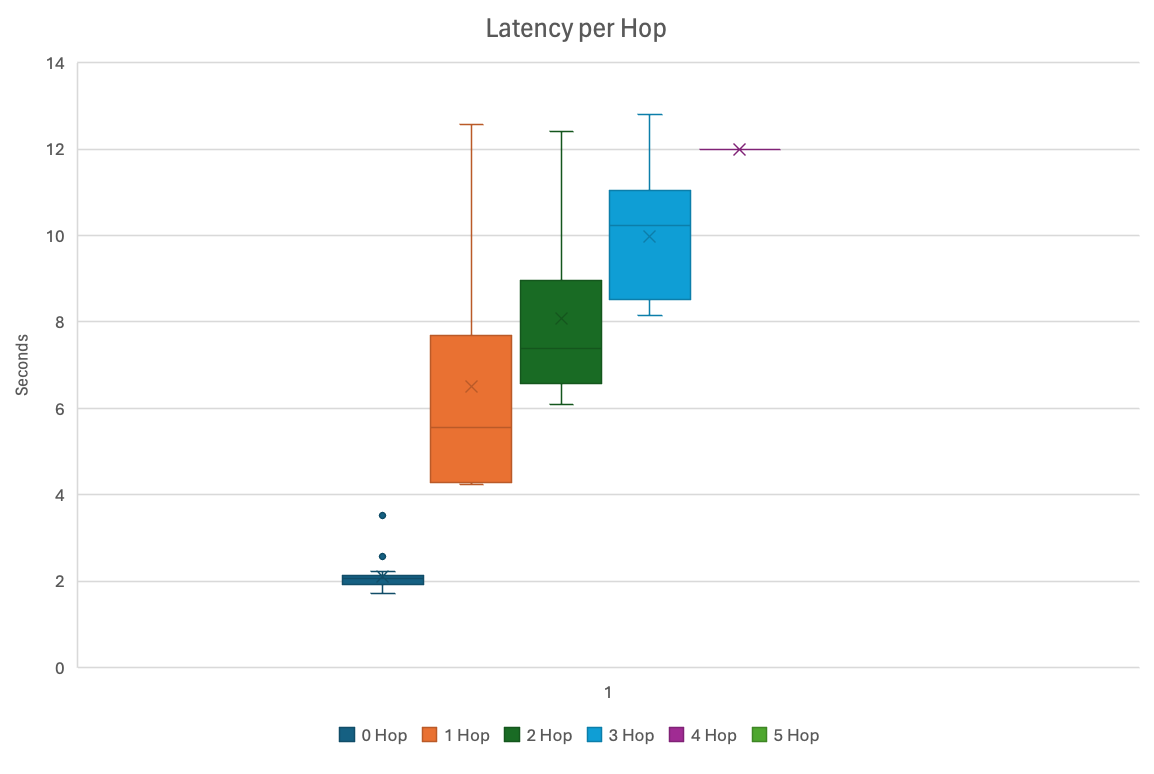
\includegraphics[width=0.7\linewidth]{images/image19.png}
    \caption{Dynamic Node Test Results - Latency per Hop}
    \label{fig:lat_per_hop}
\end{figure}

\begin{figure}[htbp]
    \centering
    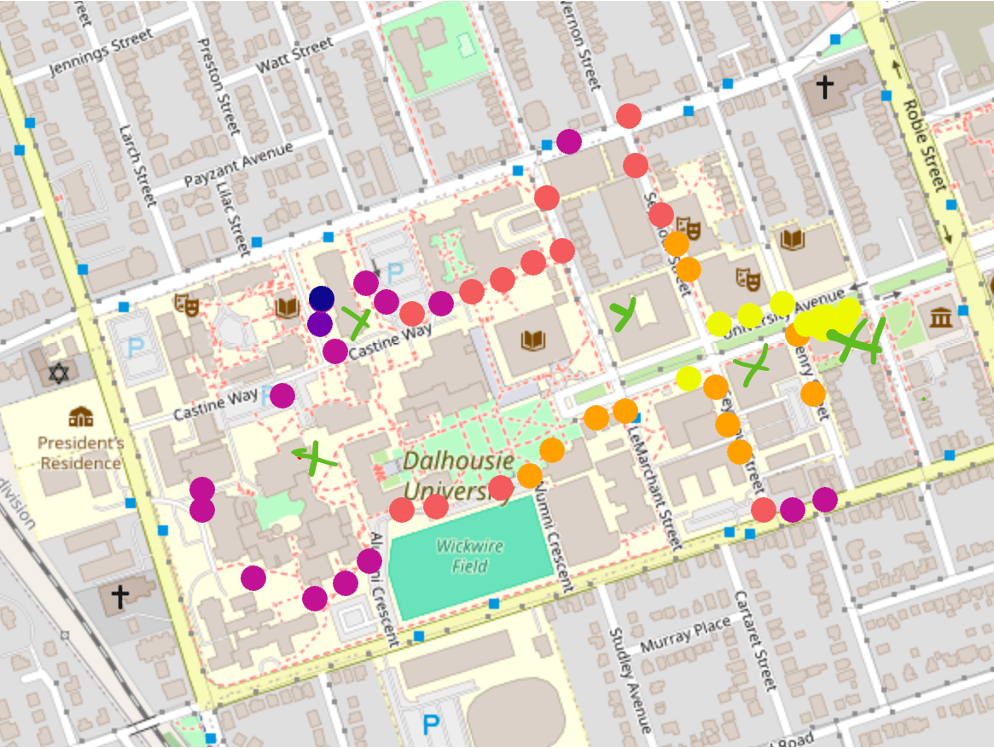
\includegraphics[width=0.7\linewidth]{images/image31.png}
    \caption{Dynamic Node Test Results - Hops by Location}
    \label{fig:hop_by_loc}
\end{figure}

\begin{figure}[htbp]
    \centering
    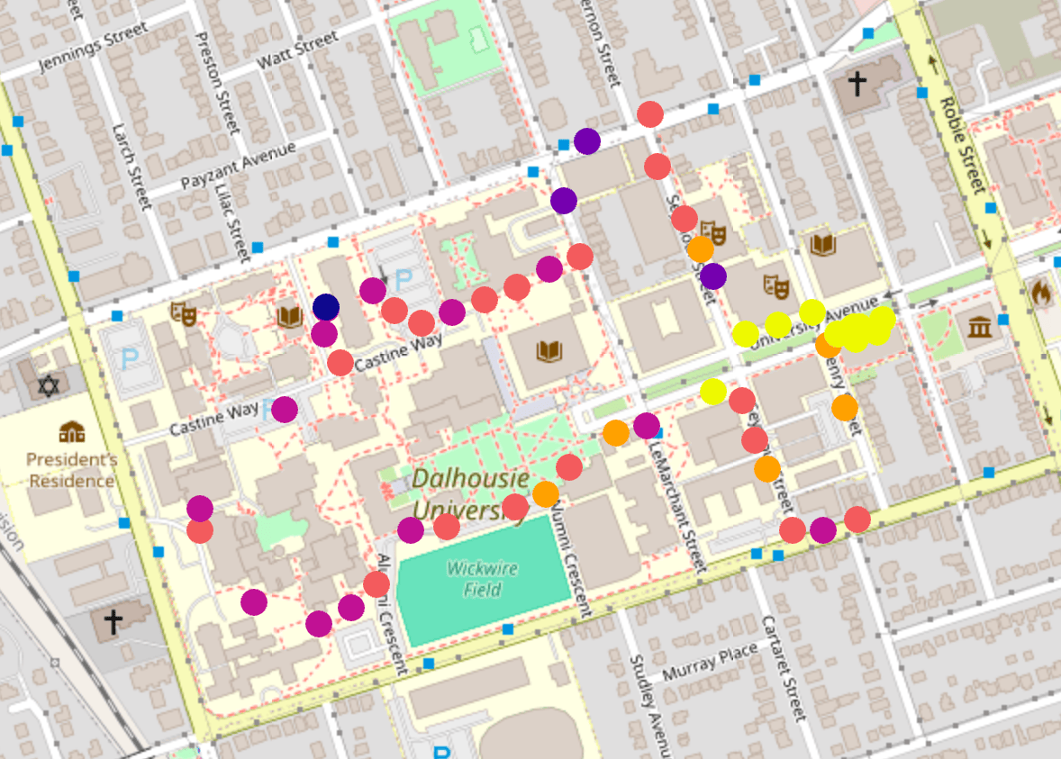
\includegraphics[width=0.7\linewidth]{images/image27.png}
    \caption{Dynamic Node Test Results - Latency by Location}
    \label{fig:lat_by_loc}
\end{figure}

Initial tests used the default hop limit of 3; however, tests were redone with the modified hop limit above, as some data was suspected to be lost when packets were not permitted enough hops to reach the destination. Unfortunately for this test, the last byte of the most recent hop was not saved. In hindsight, it would have been valuable to save this data to draw a stronger conclusion about what path was being taken, or do another set of tests entirely using Traceroute packets. 

\FloatBarrier
\subsubsection{Link Reliability Tests}

The goal of this test was to obtain data on the average spacing at which indoor nodes are placed such that they can communicate effectively. This measurement was compared with Meshtasticator simulations to determine how closely simulations matched real-world data.

For each node in the mesh, a Python script automated the sending of 50 traceroute packets at an interval of 30 seconds, recording the path taken and the SNR at each hop. The effectiveness metric used for this test was observed successful traversal rate. This was defined as the number of times a specific path occurred divided by the total number of traceroutes sent to that destination, showing how reliably the path was observed. 

\begin{equation}
    r_{ij} = \frac{N_{ij}}{N_{j}}
    \label{eq:ostr}
\end{equation}
where $r_{ij}$ is the observed successful traversal rate for link $i$ when tracing to destination $j$, 
$N_{ij}$ is the number of traceroutes to destination $j$ in which link $i$ was successfully traversed, and 
$N_{j}$ is the total number of traceroutes sent to destination $j$. $i$ represents a specific link while $j$ represents a traceroute destination.

To emphasize paths which have at least some high observed successful traversal rates, rates were weighted quadratically in their favour. 

\begin{equation}
    w_i = \sum_{j=1}^{m_i} r_{ij}^{2}
    \label{eq:ostr_rate}
\end{equation}
where $w_i$ is the weight given to link $i$ and $m_i$ is the number of observed successful traversal rates associated with link $i$. The average of these weights is defined as:
\begin{equation}
   \bar{d} = \frac{\sum_{n}^{i=1} d_i w_i}{\sum_{n}^{i=1} w_i} 
   \label{eq:weighted_distance}
\end{equation}
where $\bar{d}$ is the weighted average link distance and $d_i$ is the distance between nodes for link $i$.

Each distance was multiplied by its weight and then weighted distances were averaged. This average distance was used as the approximation for how far indoor nodes should be to communicate reliably. Only two nodes instead of the planned six in the testbed sent traceroute packets including the Goldberg 211 node and the LSC Biology 8th floor node. Sender nodes would send packets to every other node in the mesh, and a Python script was used to automate sending packets and recording how many traceroutes were sent and received. 

Based on the weights gathered for each path, the mean hop distance for all paths was 260 meters. Based on the data and formulas \eqref{eq:ostr}, \eqref{eq:ostr_rate} and \eqref{eq:weighted_distance}, two nodes placed indoors without severe blockage should be able to communicate effectively, on average, with a range of 260 meters. This estimate could be used as a baseline for any urban LoRa mesh network planning. Begin by spacing nodes at most 260 meters apart and optimize based on line of sight and propagation corridors.

\begin{figure}[htbp]
    \centering
    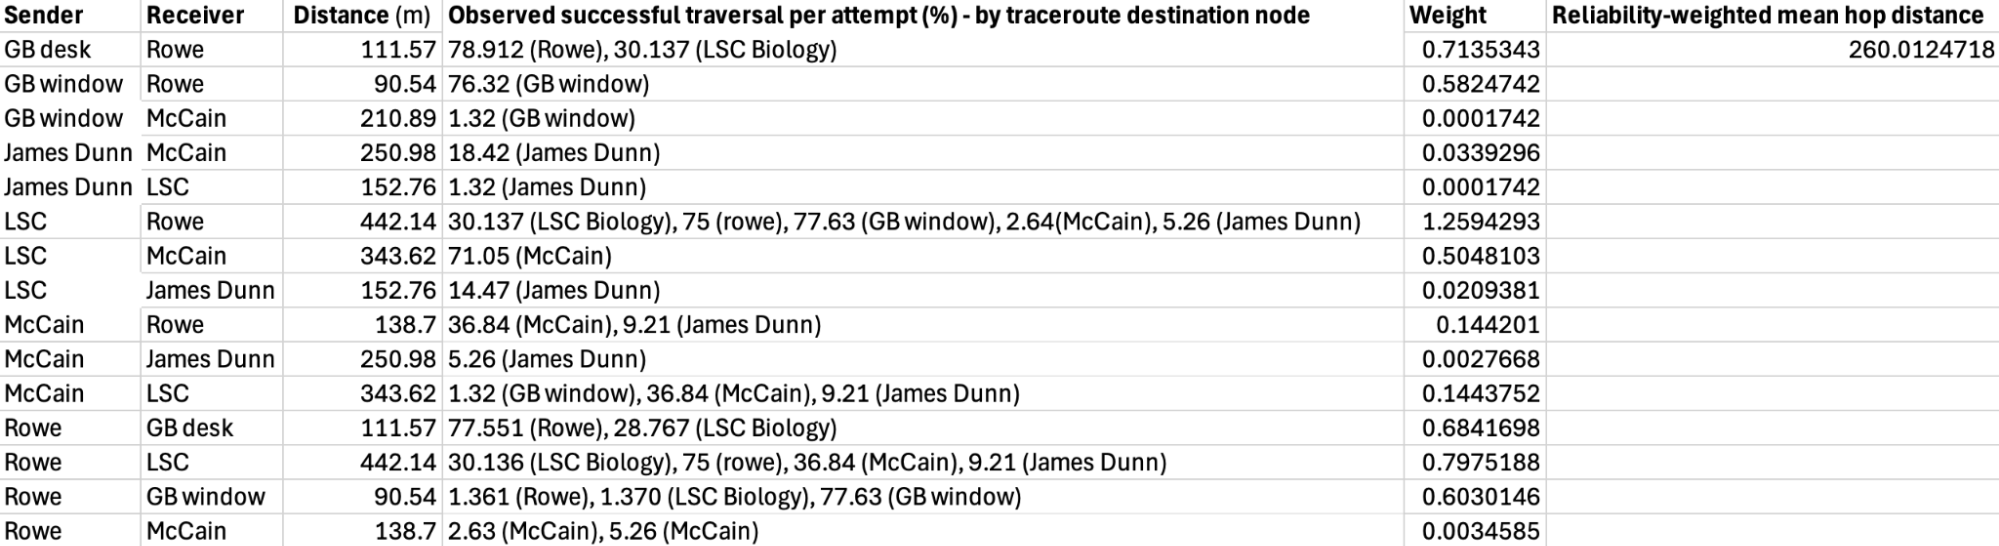
\includegraphics[width=0.7\textwidth]{images/image12.png}
    \caption{Link Reliability Test Results}
    \label{fig:link_test_results}
\end{figure}

The hardware for the test consisted only of T-Beam. All nodes were set to the default settings at the time of flashing, including a LoRa preset of LONG\_FAST and a hop limit of three.

Initial testing began with sending 50 packets every 20 seconds between different neighbours within the campus testbed. However, this proved to be overly time-consuming, and the strategy was changed to use traceroutes instead. This test was overly time-consuming, specifically during the post-test analysis. It was difficult to separate the data by traceroute destination and compute the observed successful traversal rate for each path across all destinations. It would have been much easier to use the Meshtastic range test module, while only counting indoor nodes. The time-consuming nature of the data analysis restricted this test to only two nodes. Additionally, the reliability metric of observed successful traversal rate is, ironically, not reliable as it can be easily skewed by how often it is used. It would be much more effective to measure delivery rate. However, this was not possible when using traceroute packets. Furthermore, it is unknown how effectively the weighting system eliminates the path usage bias. 

\subsection{MeshMonitor Data Collection}

Another objective was to record the busiest nodes and quantify their workload during tests and at certain times of day. Although it was attempted, a simple Python script was insufficient for this task. Thus, MeshMonitor was integrated into the mesh.

The main metrics of node behaviour in Meshtastic are stored in the local\_stats telemetry module. It gives more insight than just channel utilization including packets transmitted, packets received, packets relayed, duplicate packets received and bad packets received. MeshMonitor can scrape these metrics with a built-in automation tool and save the data into a local SQLite database. This data was visualized in Grafana, where the database was queried every thirty seconds. Each metric (other than the busiest node and battery level) is displayed as a rate per minute, as calculated in \eqref{eq:grafana_rates}. 

\begin{equation}
    R_k = \frac{M_k - M_{k-1}}{(t_k - t_{k-1})/60000}
    \label{eq:grafana_rates}
\end{equation}
where $R_k$ is the rate at sample $k$, $M_k$ is the cumulative value for the chosen metric at sample $k$ and $t_k$ is the timestamp saved for sample $k$.

The Grafana dashboard also queried device battery life by listening to standard telemetry packets and found which nodes transmitted the most packets over the past hour.

Tragically, it was not discovered until the end of the internship that instead of passively collecting data on the behaviour of the mesh over time, MeshMonitor was deleting old telemetry data. Thus, the latest snapshot of the dashboard only has local\_stats telemetry data from July 31st 5 p.m. 

\begin{figure}[htbp]
    \centering
    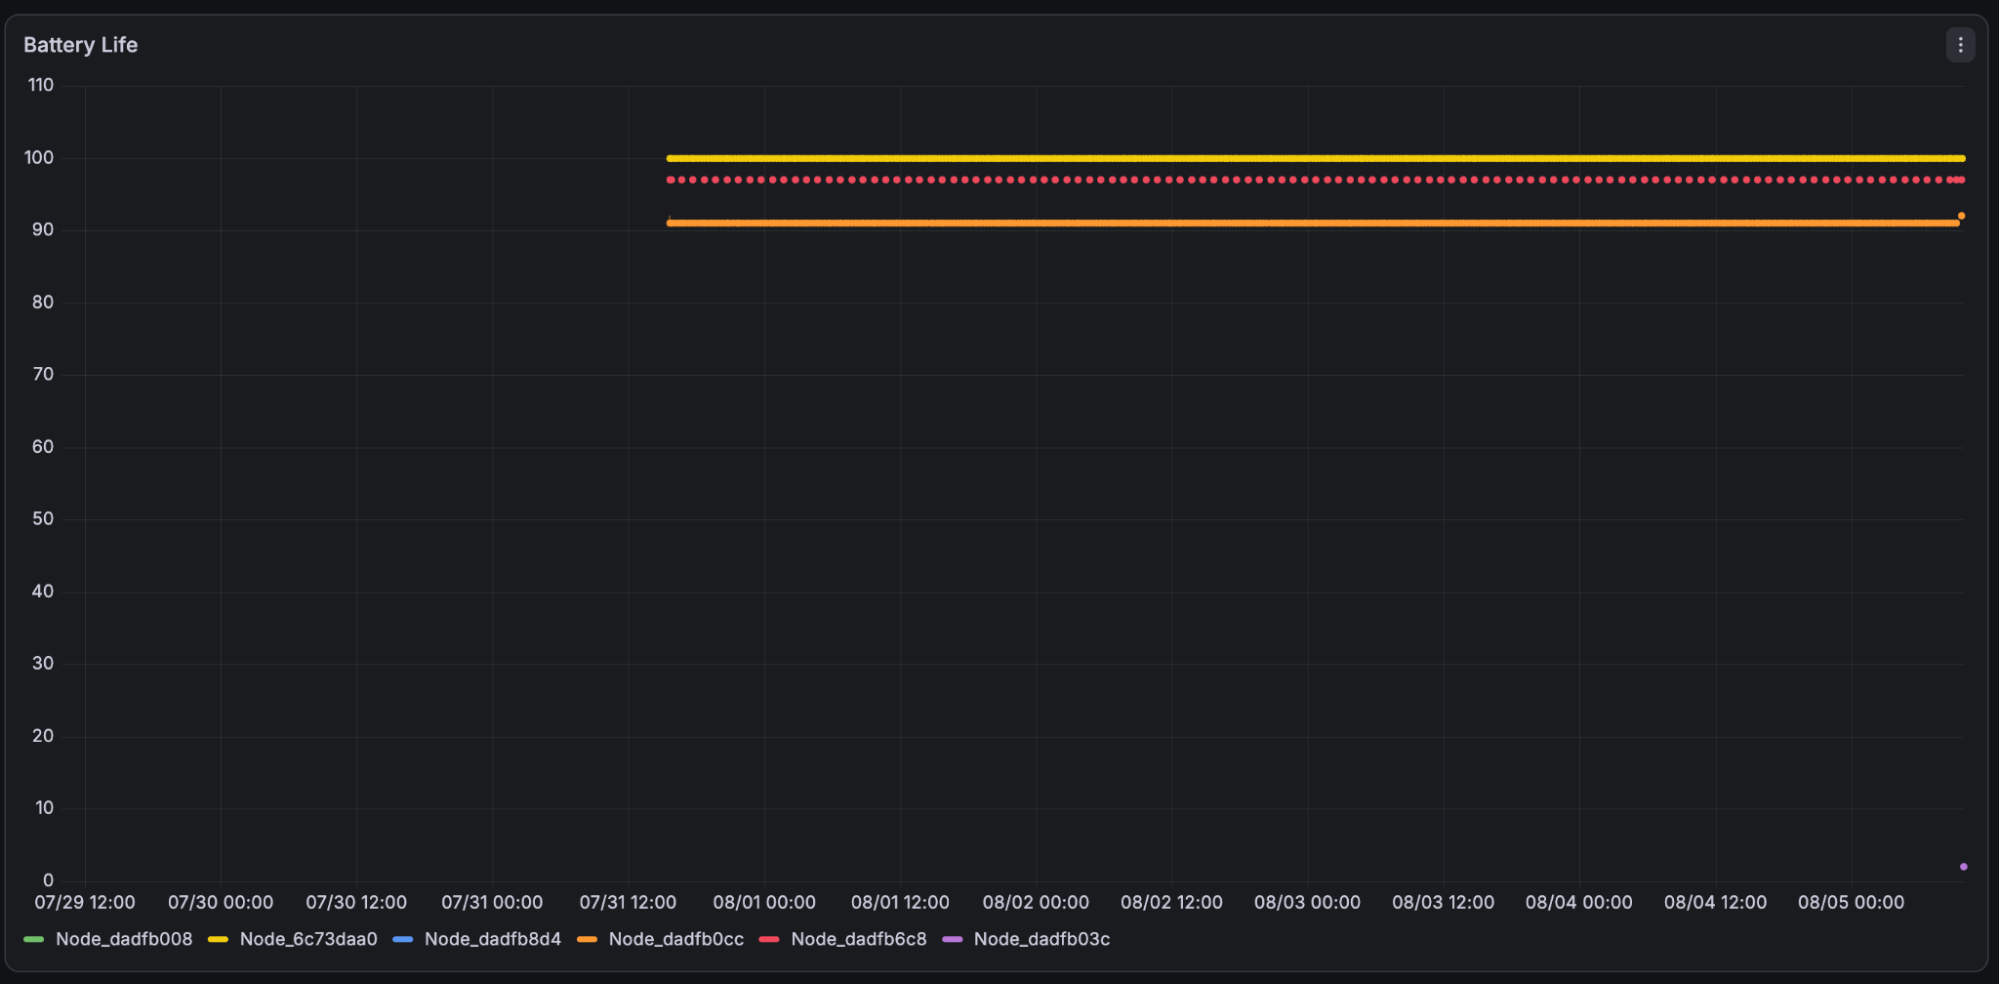
\includegraphics[width=0.7\textwidth]{images/image36.png}
    \caption{Battery Life Monitor}
    \label{fig:battery}
\end{figure}

\begin{figure}[htbp]
    \centering
    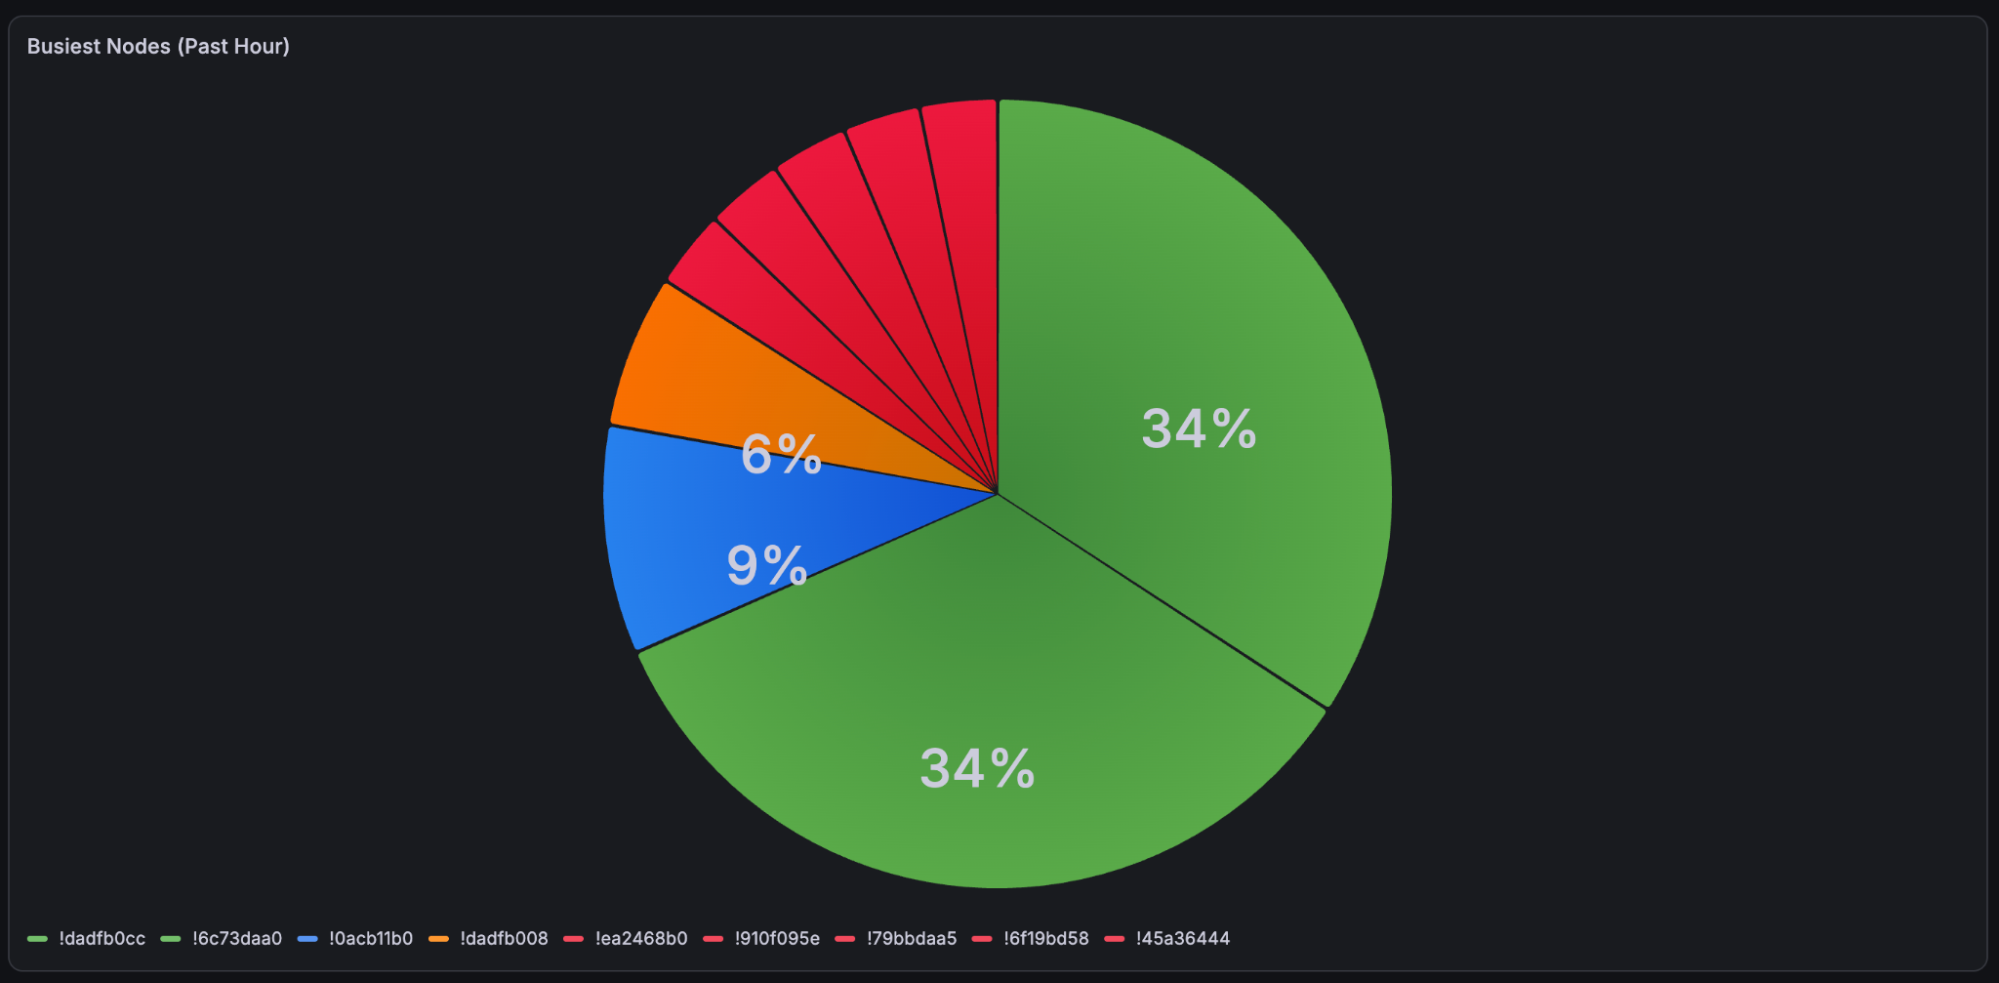
\includegraphics[width=0.7\textwidth]{images/image23.png}
    \caption{Busiest Node Monitor}
    \label{fig:busiest_node}
\end{figure}

\begin{figure}[htbp]
    \centering
    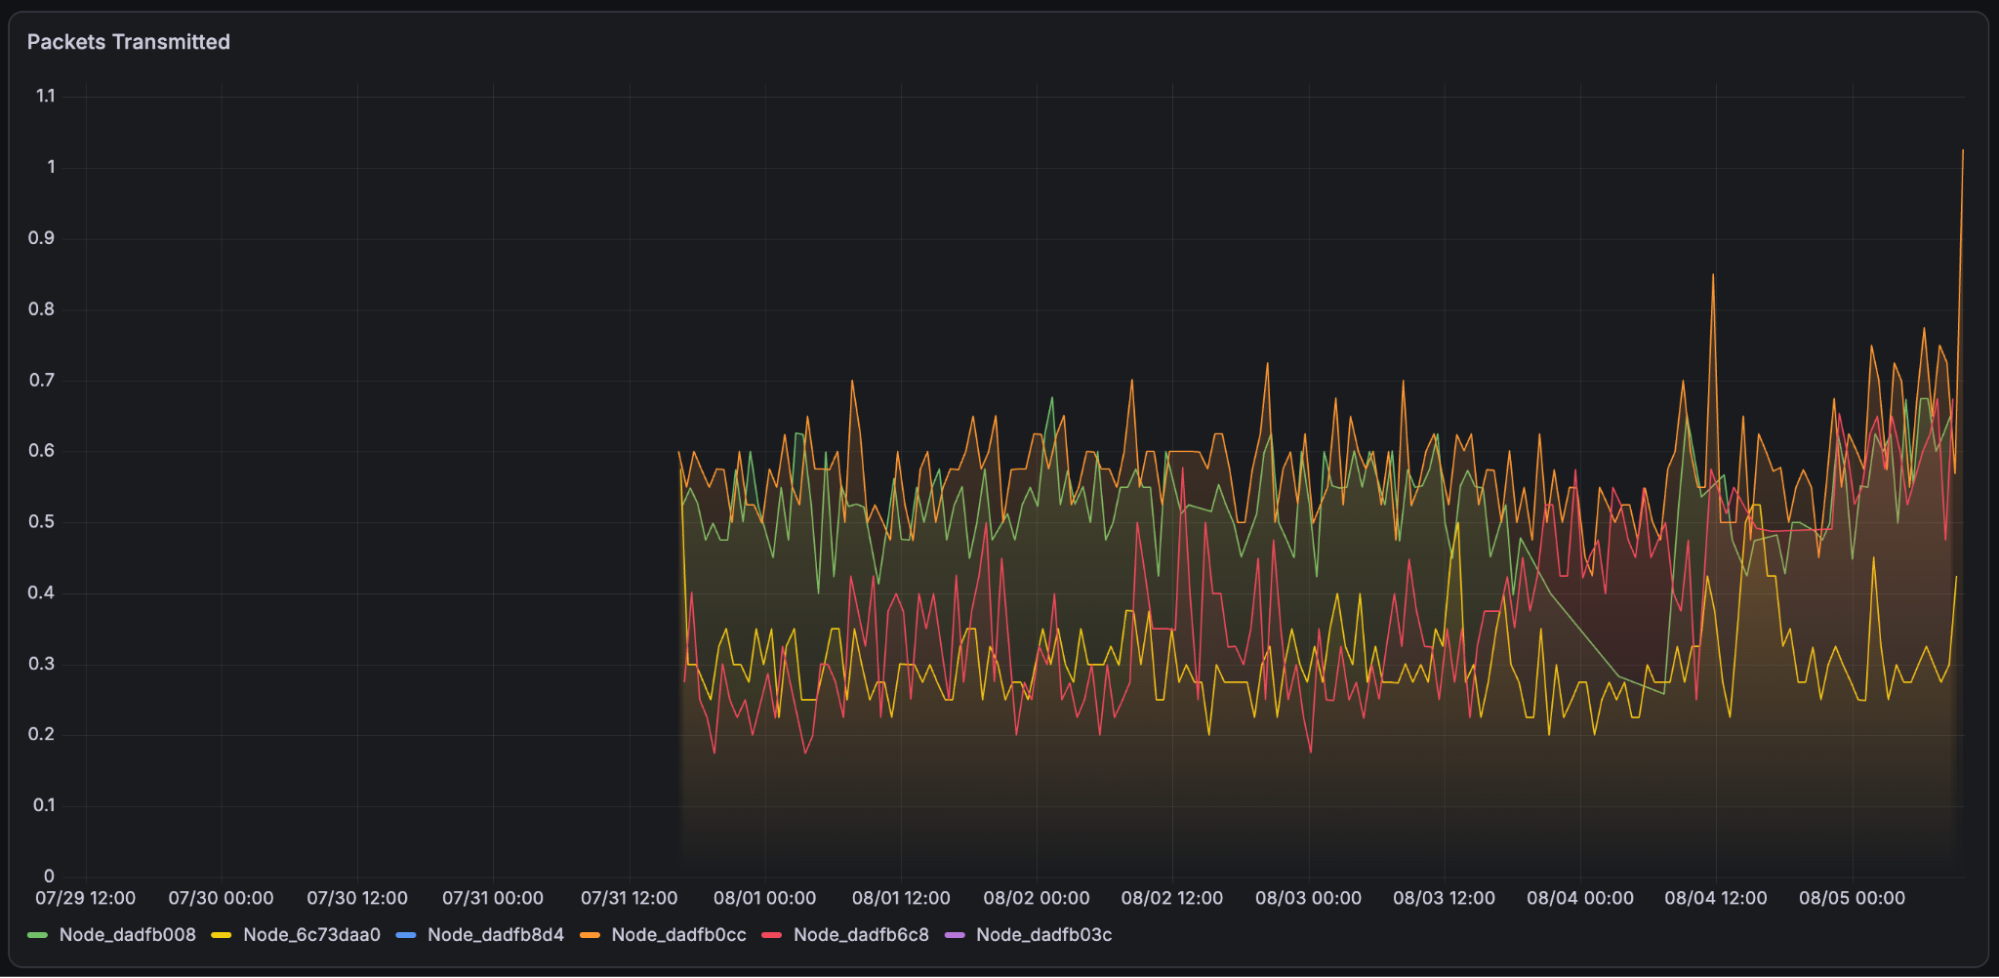
\includegraphics[width=0.7\textwidth]{images/image21.png}
    \caption{Packets Transmitted Monitor}
    \label{fig:packets_tx}
\end{figure}

\begin{figure}[htbp]
    \centering
    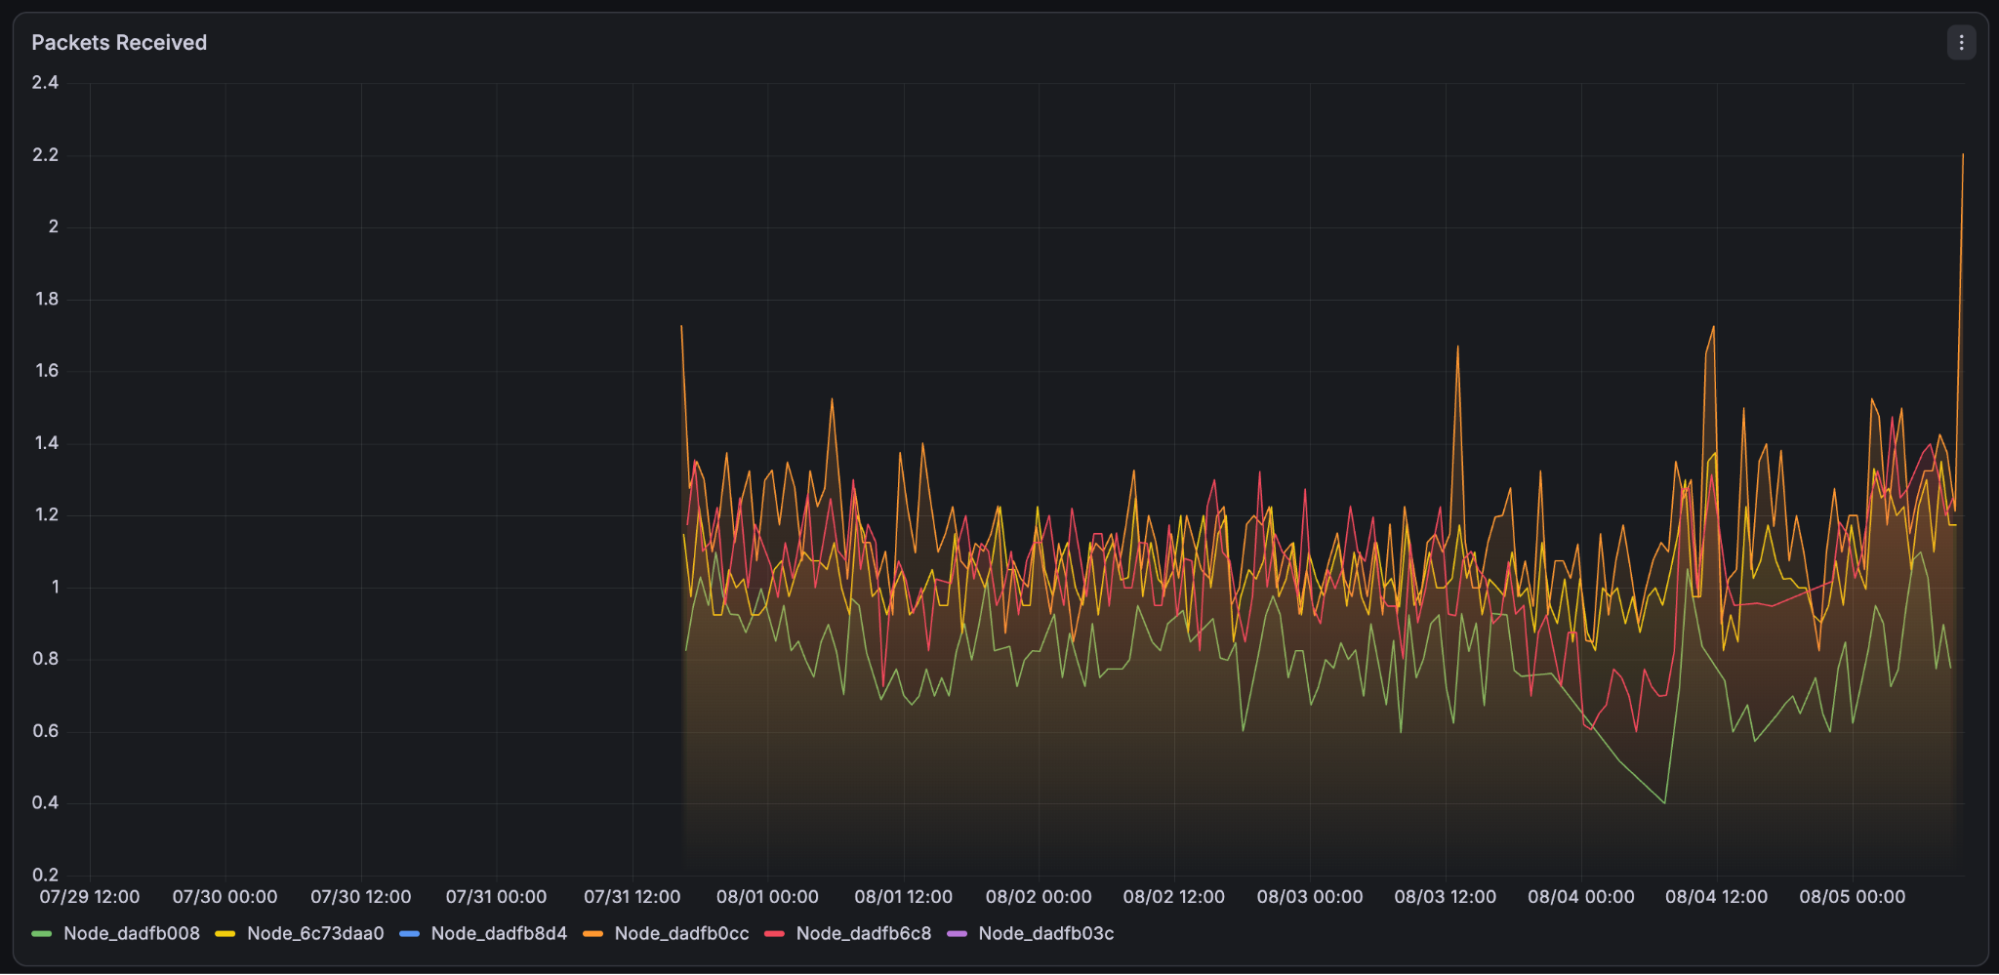
\includegraphics[width=0.7\textwidth]{images/image25.png}
    \caption{Packets Received Monitor}
    \label{fig:packets_rx}
\end{figure}

\begin{figure}[htbp]
    \centering
    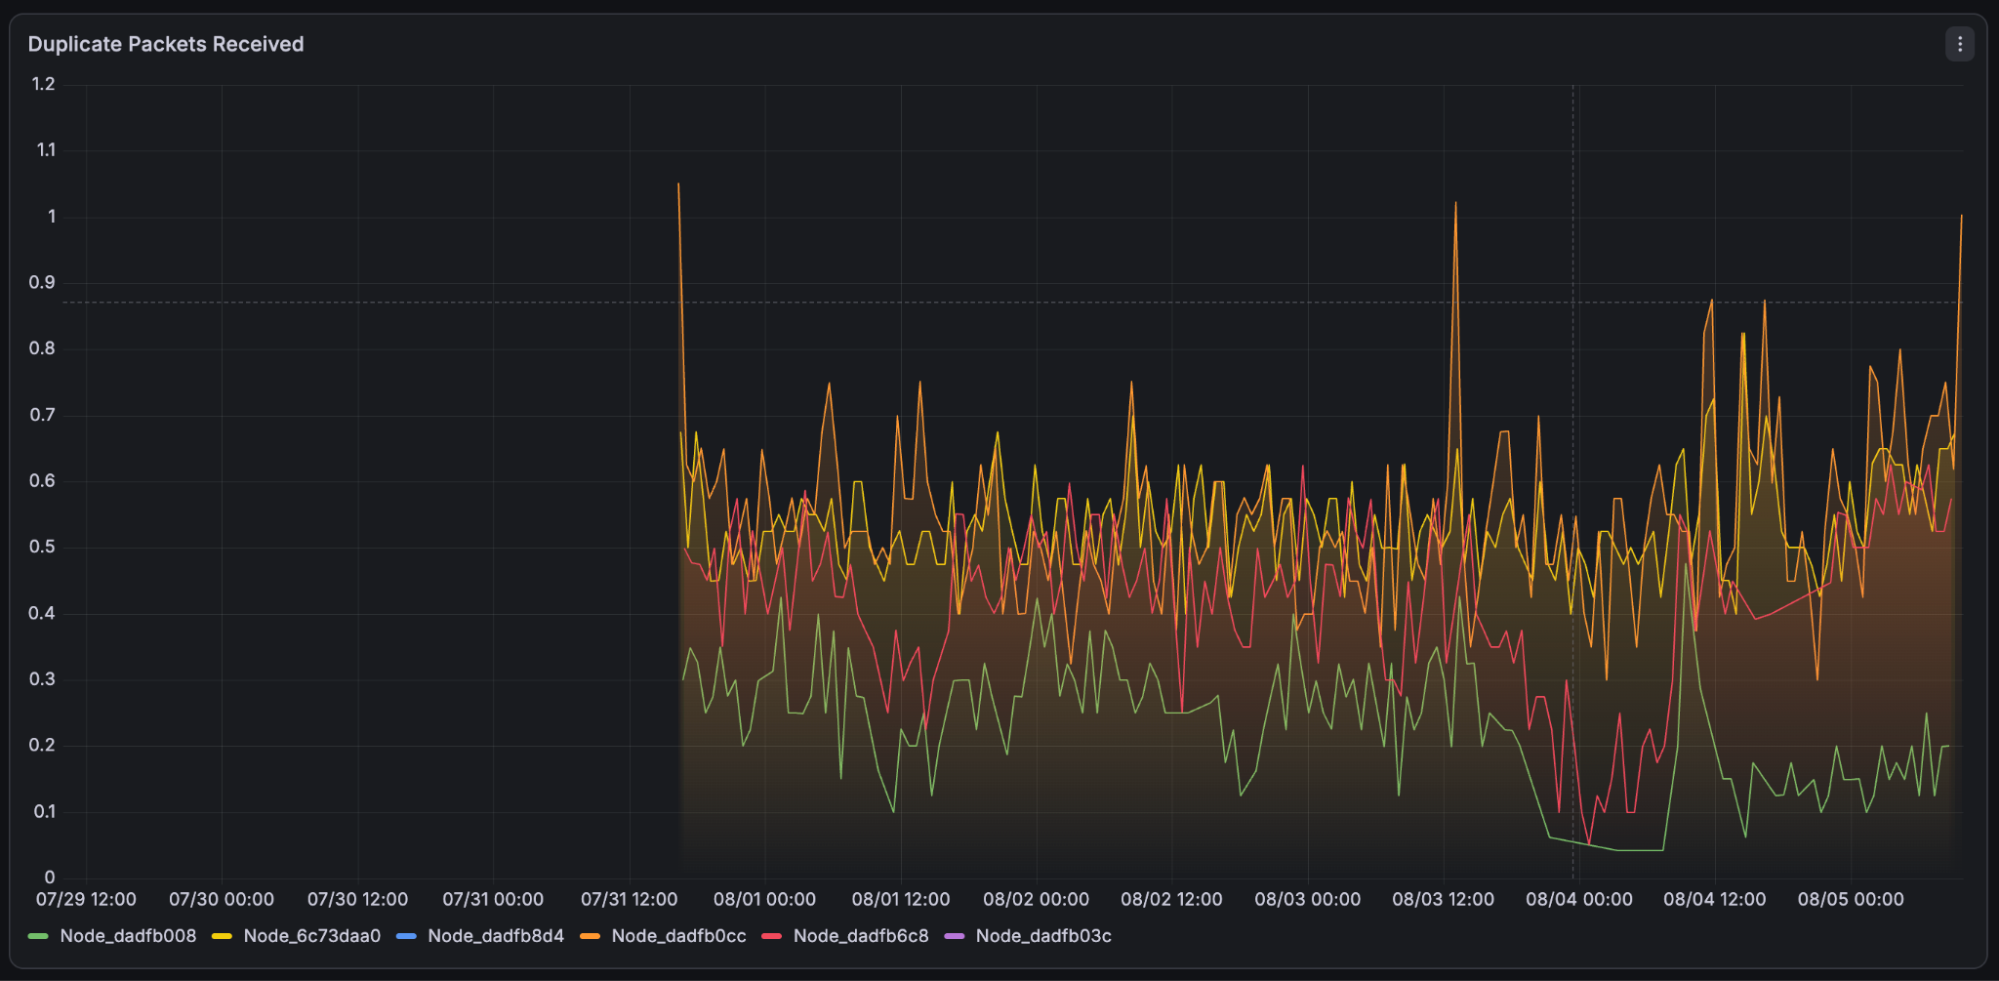
\includegraphics[width=0.7\textwidth]{images/image28.png}
    \caption{Duplicate Packets Received Monitor}
    \label{fig:packets_dup_rx}
\end{figure}

\begin{figure}[htbp]
    \centering
    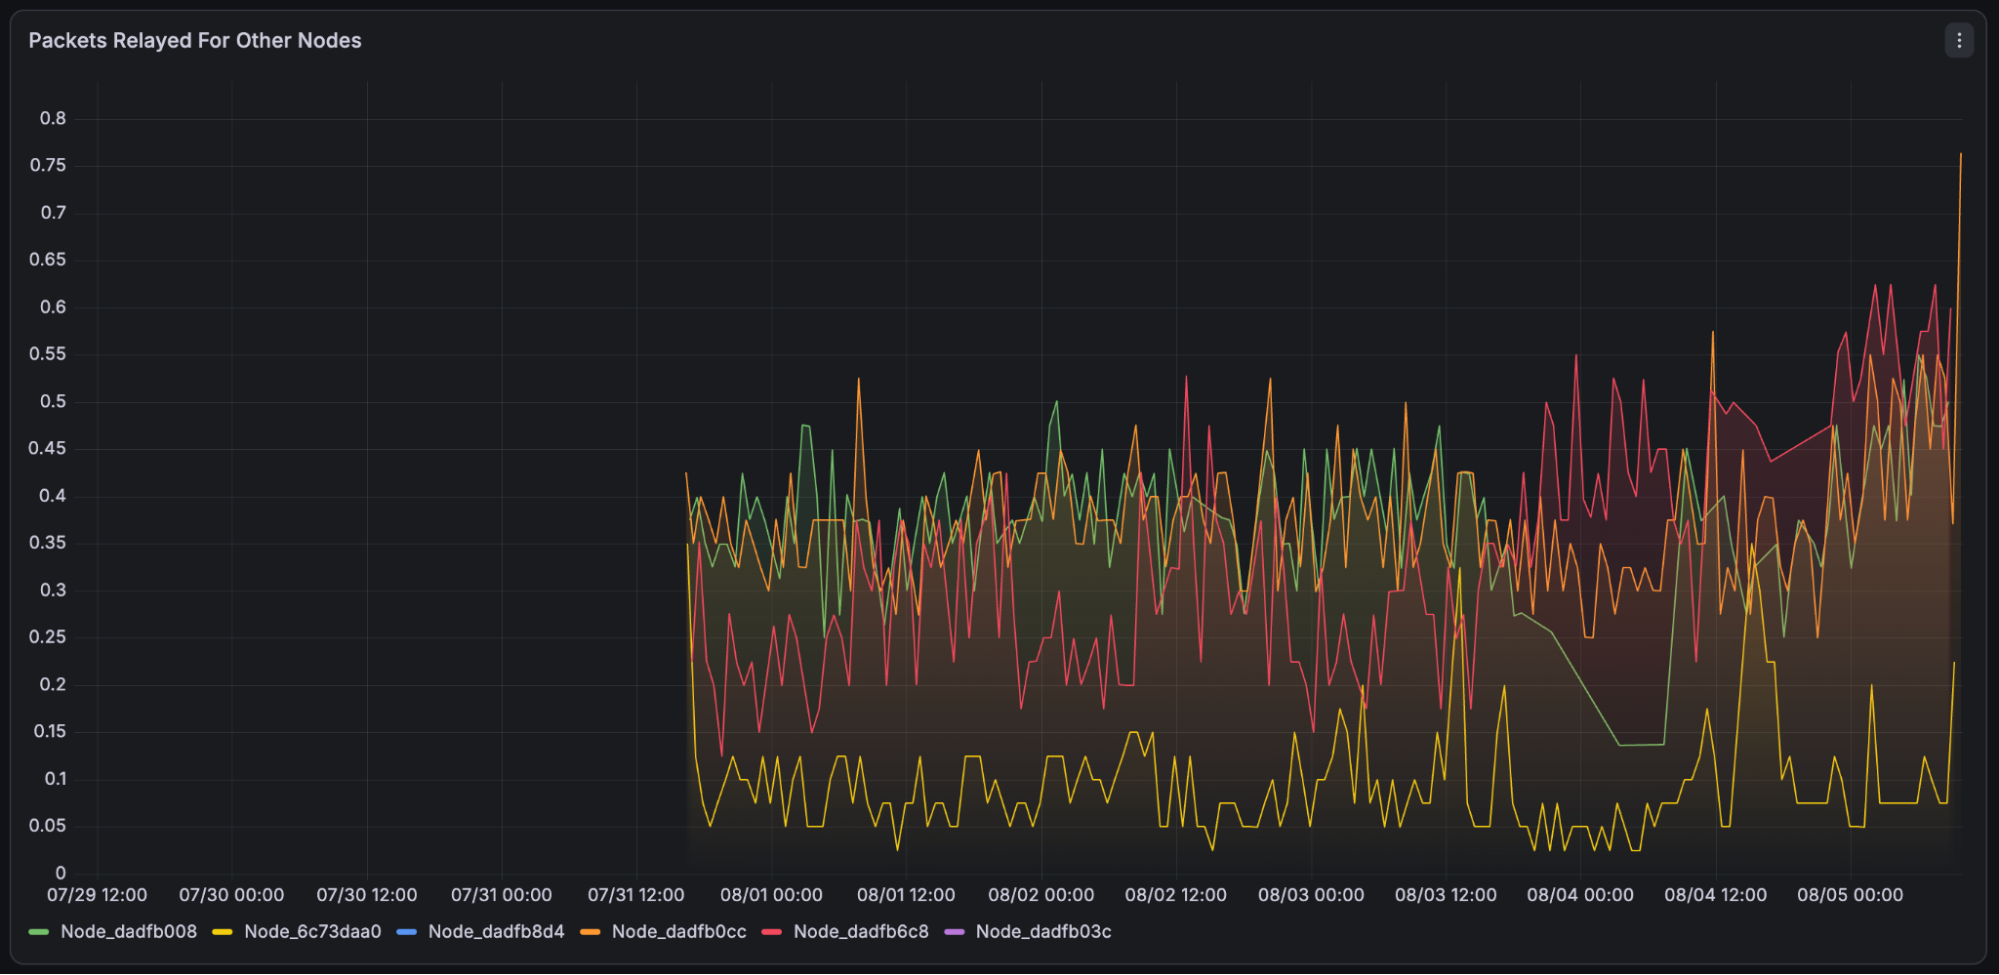
\includegraphics[width=0.7\textwidth]{images/image34.png}
    \caption{Packets Relayed Monitor}
    \label{fig:packets_relayed}
\end{figure}

From the data available, it seems that nodes !dadfb008 (LSC Biology 8th floor) and !dadfb0cc (Rowe 5001) not only transmit the most packets but also receives the most packets. This is understandable as they are the best positioned nodes in terms of line of sight and elevation. The packet reception rate seems to be similar across all nodes, except the Rowe node seems to have occasional spikes in activity. The cause of this is unknown, possibly because it connects to the most nodes in the mesh including the LSC, both Goldberg nodes and occasionally McCain. The LSC node has the highest bad packet rate, which is understandable as it has the highest elevation and best reception range, thus introducing more noise. The Rowe and Goldberg 211 (!6c73daa0) nodes have the highest duplicate packet rate, likely because they are within close proximity to each other. 

Although the busiest nodes for that hour were the Goldberg window and Rowe nodes, this metric can change drastically at any given point. The other two nodes, !dadfb03c (James Dunn) and !dadfb8d4, are not shown because !dadfb8d4 is not active, and !dadfb03c was running on battery power and had been drained. In summary, a mesh of this scale (5-6 nodes) does not have to work hard to stay active. Nodes are often transmitting packets anywhere from 0.2 to 0.7 packets per minute, rarely exceeding 1 packet per minute. This shows there is no concern about congestion for a mesh of this size, and there is little outside activity that the mesh has been contributing to. In a city the size of Halifax, this is healthy; however, in a large metropolitan area with many more outside contributors, a mesh of this size will likely have to work much harder. It is important to monitor these metrics as nodes with the highest traffic are likely to have the greatest battery consumption and channel utilization. When building a LoRa mesh network, prioritizing these nodes for improved antennas, increased power supplies or dedicated relay roles will help to increase the performance of the mesh as a whole.

\FloatBarrier
\subsection{Meshtasticator Simulations}

\subsubsection{Halifax Peninsula}

The initial goal of these tests was to estimate the scale at which a Meshtastic network in Halifax would perform best. However, initial tests showed interesting results, many of which were difficult to understand. For this reason, more simulations with simpler conditions were conducted to determine the cause of the initial results.

Simulations were conducted using the community software Meshtasticator. Meshtasticator is an open-source discrete-event and interactive simulator for Meshtastic LoRa networks written in Python. It simulates the behaviour of a Meshtastic network, including packet transmission, propagation, collision and routing without the need for hardware. Meshtasticator is a simple simulator that does not account for buildings, terrain and interference. The only way it compensates for these factors is by applying one of six path loss models, each one for a different environment. While Meshtasticator supports random node placement within a quadrilateral, it does not support complex shapes like the Halifax peninsula. To accommodate this, the Meshtasticator repository was forked and modified to allow the user to give a polygon as a GeoJSON file and then randomly generate coordinates within the polygon. Unlike the default Meshtasticator behaviour, which ensures a node is always connected to at least one other node before placing, this custom logic is closer to true randomness. 

Metrics gathered include network reach (\%), mean message delay (milliseconds), collision rate (\%), transmit airtime utilization (\%), transmissions per message (i.e.,  transmission overhead), useful receptions (\%), and mean minimum node distance (meters). These metrics are defined by Equations~\eqref{eq:network_reach}, \eqref{eq:mean_message_delay}, \eqref{eq:collision_rate}, \eqref{eq:tx_airtime_util}, \eqref{eq:tx_per_msg} and \eqref{eq:mean_min_mode_distance}

\begin{equation}
    \text{Network Reach} =
    \frac{N_{\text{useful receptions}}}
    {N_{\text{messages created}}(N_{\text{nodes}} - 1)}
    \times 100
    \label{eq:network_reach}
\end{equation}

\begin{equation}
    \text{Mean Message Delay} =
    \frac{\sum (t_{\text{reception}} - t_{\text{generation}})}
    {N_{\text{successfully received packets}}}
    \label{eq:mean_message_delay}
\end{equation}

\begin{equation}
    \text{Collision Rate} =
    \frac{N_{\text{collided packets}}}
    {N_{\text{sensed packets}}}
    \times 100
    \label{eq:collision_rate}
\end{equation}

\begin{equation}
    \text{Transmit Airtime Utilization} =
    \frac{t_{\text{total transmission airtime}}}
    {t_{\text{simulation}}}
    \times 100
    \label{eq:tx_airtime_util}
\end{equation}

\begin{equation}
    \text{Transmissions per Message} =
    \frac{N_{\text{total packet transmissions}}}
    {N_{\text{unique messages created}}}
    \label{eq:tx_per_msg}
\end{equation}

\begin{equation}
    \text{Mean Minimum Node Distance} =
    \frac{\sum_{i=1}^{N_{\text{nodes}}} d_i}
    {N_{\text{nodes}}}
    \label{eq:mean_min_mode_distance}
\end{equation}
where $d_i$ is the distance to node $i$'s nearest neighbor. These results are grouped by number of nodes, and are displayed as the mean for each group.

Simulations were repeated multiple times for different node counts and hop limits. Each batch of simulations had 220 simulations total, with 20 simulations conducted for each node count. The node counts included 5, 7, 10, 12, 14, 17, 22, 32, 52, 77 and 102 nodes. Two of the nodes in the simulation are fixed: one at the top of the peninsula and one at the bottom. For the first batch, messages had a hop limit of 3, while the second batch had a hop limit of 7. Configuration settings were set to make conditions as realistic as possible. These changes included the antenna gain of the node, the transmit power and the path loss model, set to 2 dB, 20 dBm, and 3GPP (metropolitan), respectively. The Halifax polygon was taken by mapping the coastline, then using Joseph Howe Drive as a boundary to separate the peninsula from the mainland.

The Halifax mesh simulation with a 7-hop limit had far better network reach; however, it came at a high cost. The cause for the sudden decrease in network reach is likely due to collisions and congestion decreasing useful receptions in conjunction while the number of nodes increases. In the network reach formula \eqref{eq:network_reach}, the numerator is slowly decreasing while the denominator increases sharply.
\begin{figure}[htbp]
    \centering
    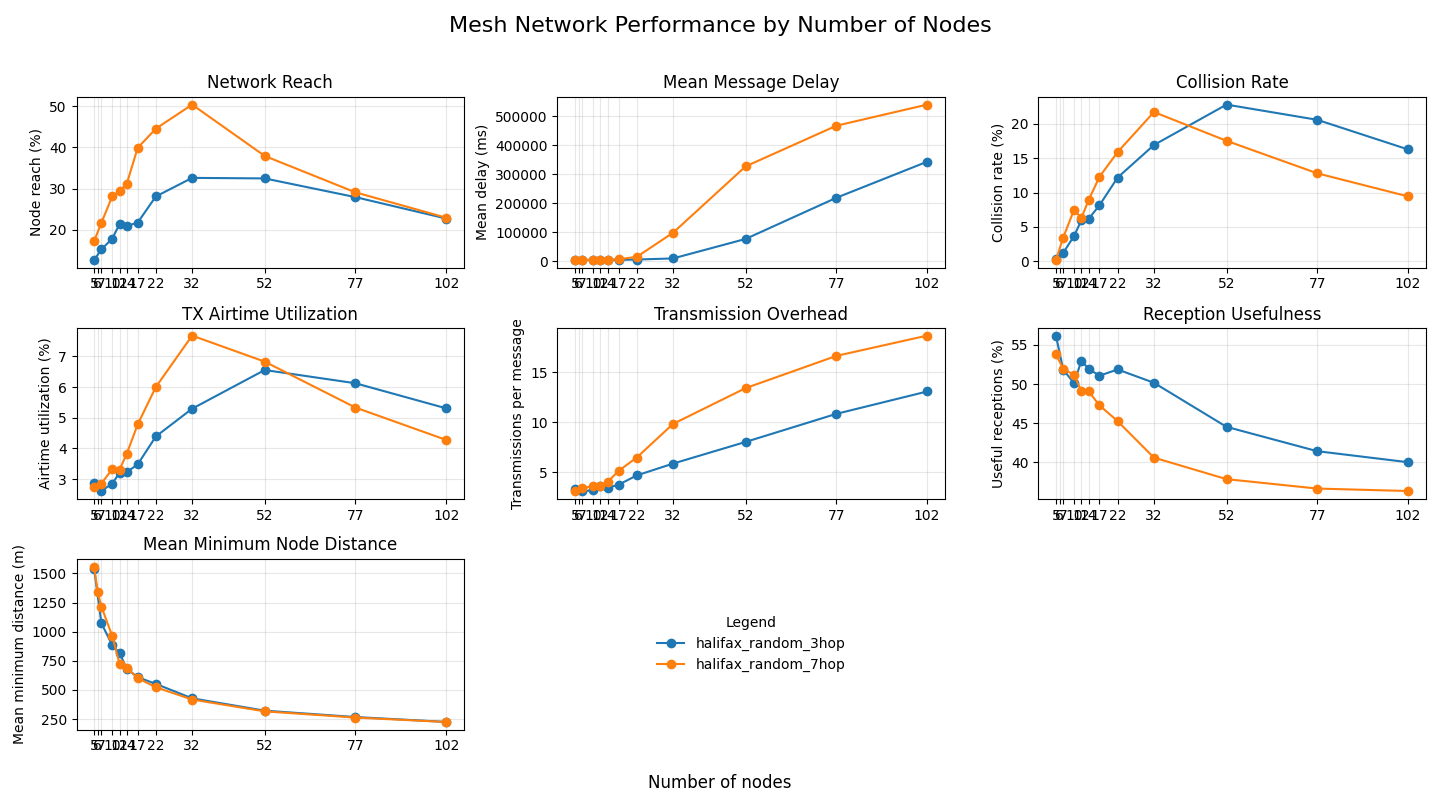
\includegraphics[width=0.7\textwidth]{images/image15.png}
    \caption{Halifax Meshtasticator Simulation Results}
    \label{fig:halifax_sim}
\end{figure}
On almost all other metrics, the 7-hop mesh performs more poorly than the 3-hop mesh. At 22 nodes and below, the mean message delay is essentially zero for both the 7-hop and 3-hop meshes. However, past 22 nodes, the delay of the 7-hop is about double that of the 3-hop, with the former exceeding the latter by over 200,000 ms or 3$\frac{1}{3}$ minutes. Both the 3-hop and 7-hop meshes reach a peak collision rate of 20\%. However, the 3-hop mesh reaches this limit at 52 nodes. The reason for the decrease in collision rate is that the number of nodes is increasing faster than the number of collisions, thus decreasing the collision rate. 
\begin{figure}[htbp]
    \centering
    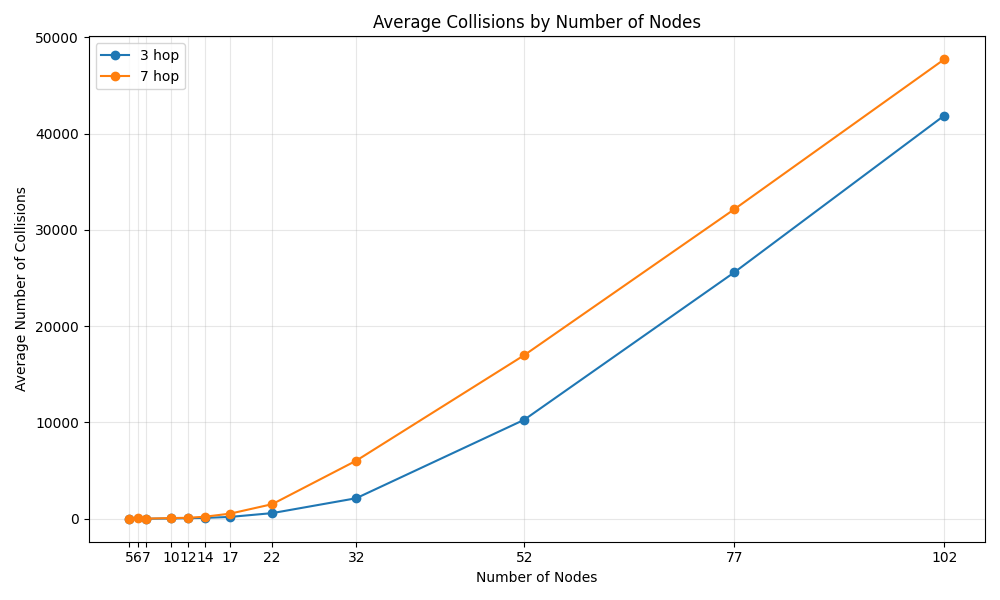
\includegraphics[width=0.7\textwidth]{images/image24.png}
    \caption{Halifax Simulation - Average Collisions}
    \label{fig:halifax_collisions}
\end{figure}

The airtime utilization rate shows similar behaviour to the collision rate. However, upon close inspection of the transmission airtime in seconds, there is unusual behaviour where the 7-hop mesh begins higher than the 3-hop, but later falls below it. 
\begin{figure}[htbp]
    \centering
    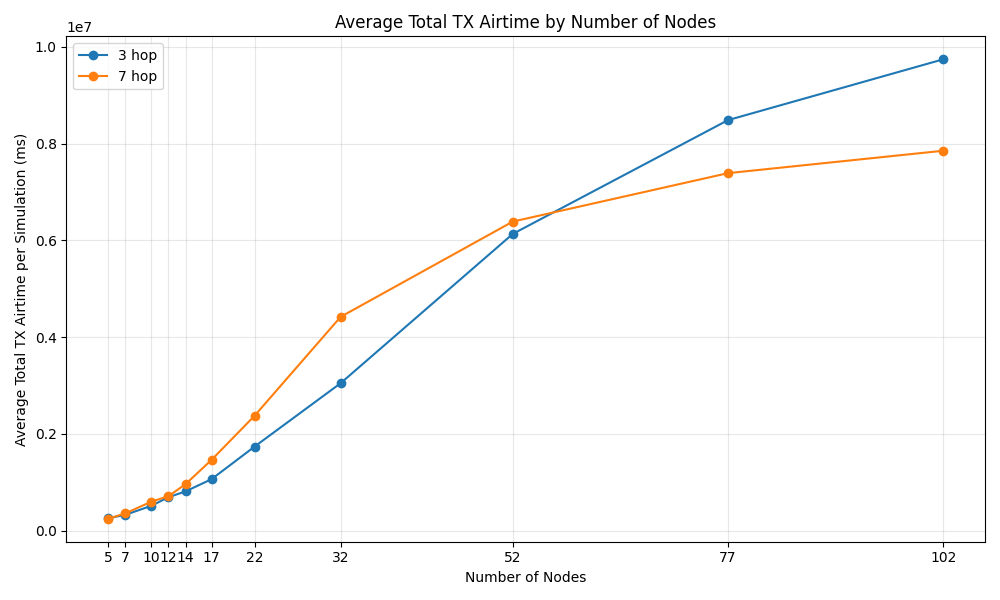
\includegraphics[width=0.7\textwidth]{images/image10.png}
    \caption{Halifax Simulation - Average Transmit Airtime}
    \label{fig:halifax_tx_airtime}
\end{figure}
The most plausible explanation for this trend is that at this point, the 7-hop mesh is too congested and packets cannot be rebroadcast because nodes are waiting for access to the channel. At some point, nodes may wait so long to broadcast that the simulation will end before the rebroadcast can be sent, thus decreasing the transmit airtime. This behaviour can be investigated further by examining the ratio of the number of packets sent, which includes all retransmissions, to the number of unique messages created.
\begin{figure}[htbp]
    \centering
    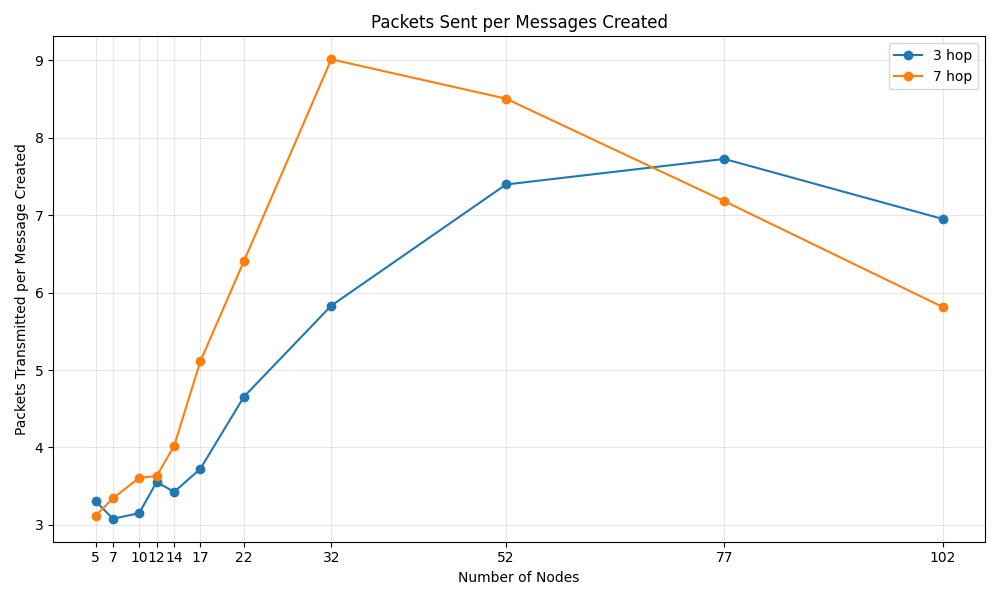
\includegraphics[width=0.7\textwidth]{images/image30.png}
    \caption{Halifax Simulation - Packages Sent per Message}
    \label{fig:halifax_package_per_message}
\end{figure}
Figure~\ref{fig:halifax_package_per_message} shows that the 7-hop mesh increases in packets transmitted per created message much more quickly than the 3-hop mesh. However, it reaches congestion earlier, and consequently the number of packets transmitted per message decreases earlier as well. This also explains the high mean message delay after 32 nodes for the 7-hop mesh or 52 nodes for the 3-hop mesh. Once the mesh becomes congested nodes begin contending for channel use, increasing the wait time before a message can be sent.

Continuing with other trends, transmission overhead is far higher with the 7-hop mesh than the 3-hop mesh, as expected. Reception usefulness is lower for the 7-hop mesh, which is understandable for a dense mesh, as the number of duplicate packets will increase as the extra hops are being used for previously seen nodes. The increase in network reach with a decrease in performance shows that, for an area the size of Halifax, a 7-hop mesh has better network reach, but this propagation is far less efficient. Comparing other metrics to the mean minimum node distance, a proxy for node density, it seems that routing efficiency and performance begin to degrade at just over 418 meters for 7-hop meshes and around 322.73m for 3-hop meshes. This is a 26\% increase over the 260 meters 3-hop range estimate obtained from data collected in the Dalhousie Meshtastic testbed. The results show that increasing hop limits may not always be beneficial. Depending on the density of nodes, a higher hop limit may significantly reduce network efficiency or increase congestion, while barely improving network reach.

\FloatBarrier
\subsubsection{Square Area Validation Test}

Initial results from the test above were misleading as there was a misalignment between the header and the data in the CSV files. This caused highly unusual activity which could not be explained. Before this error was found, a baseline simulation was done with the same number of nodes and repetitions as above, but with the polygon set to a 1,000 meter by 1,000 meter or a 2,000 meter by 2,000 meter square. Both test groups used a hop limit of 7.
\begin{figure}[htbp]
    \centering
    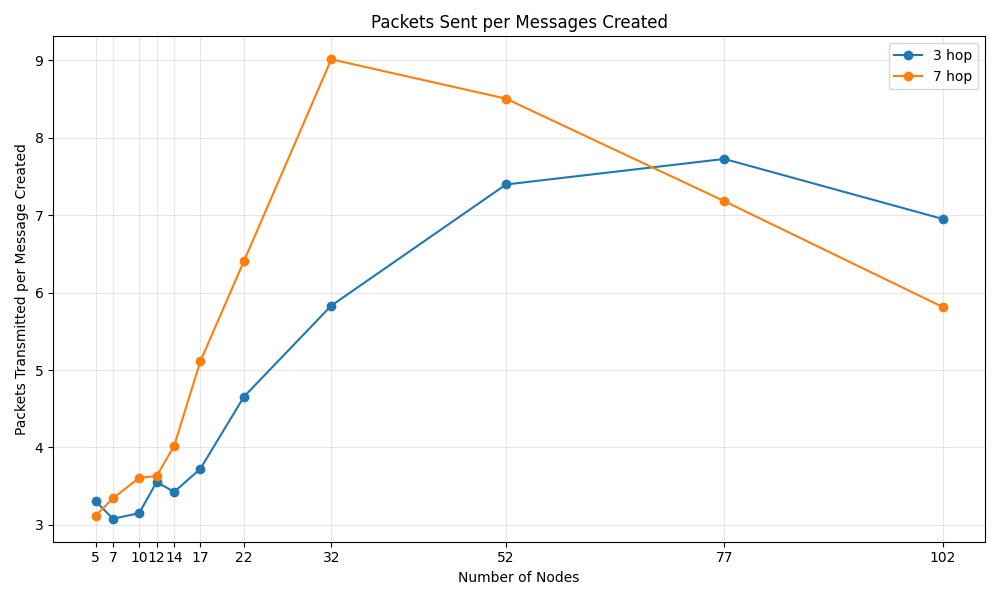
\includegraphics[width=0.7\textwidth]{images/image30.png}
    \caption{Square Area Validation Test Results}
    \label{fig:square_results}
\end{figure}

Many of the metrics in Figure~\ref{fig:square_results} are nearly identical for the 1,000 meter area and 2,000 meter area aside from collision rate and transmit airtime. The network reach shows similar behaviour to the Halifax test, with the sudden decrease likely attributed to a decrease in useful receptions in proportion to a large increase in the number of nodes. Mean message delay also skyrockets as congestion increases, however, at similar paces. The extreme difference in collision rate between the 1,000 meter and 2,000 meter boxes is oddly caused by the density of the nodes. Because 30 nodes are denser in the 1,000 meter box, the mesh becomes congested more quickly and contention over the use of the channel begins earlier. Nodes are likely waiting to send messages before collisions can occur because of the high density. This is also the cause of the difference in transmission airtime between the two areas. The reception usefulness rate is generally higher for the 2000m node area, not because there are more useful receptions, but because the number of packets received for the 1,000 meter area far exceeds the 2,000 meter area. Sampling all points where the node count is 32, the average useful receptions for 1,000 meter and 2,000 meter simulations is 8,498 and 7,345, respectively. The average total packets received for 1,000 meter and 2,000 meter simulations is 33,385 and 24,739 respectively. This brings the reception usefulness rate to 25.5\% for the 1000m area and 29.7\% for the 2,000 meter area. This trend continues for all node counts.

\FloatBarrier
\section{Discussion}

Despite all the tests and simulations conducted throughout the internship, it is difficult to provide a definitive answer to the question: can Meshtastic be used reliably and effectively in an urban environment? A core part of what makes this question difficult is how to define reliability and effectiveness. At what rate or level does one determine that communication is reliable, and at what scale is this possible? However, within the scope of this study, results indicate that effective urban communication using Meshtastic is possible, but only at a small scale. It could not be used as an emergency communication system for the general public and would be unpredictable for a small subset of the population, for example, emergency responders.
	
The range tests effectively demonstrated how buildings and obstructions affect performance. The SMU field tests showed consistent, reliable communication up until the point of going behind one set of buildings, about 220 meters away. RSSI dropped from -100 to under -120 after one obstruction, showing how only one building can be the difference between reliable communication and pushing the sensitivity barrier. Halifax bike tests further contributed to this claim, as long-range communication past 250m was usually only possible when a node was placed directly on a corresponding street with negative elevation. In this case, communication was found to be possible up to 1.1 kilometers. Therefore, maximizing the performance of urban communication using Meshtastic requires the use of streets as propagation corridors.

The Dalhousie Meshtastic testbed provided insights into how resilient the managed flooding routing protocol is to dynamic nodes and how adding hops impacts latency and delivery rate. The stable route test from the Goldberg window node to the Dalplex showed that on just one path, assuming there was little background activity from other nodes, sending messages at a five-second interval would cause collisions, causing the delivery rate to drop to an average of 30\%. However, in an area where there is high background activity on the same channel, longer intervals may have the same effect. Furthermore, it showed that every hop adds approximately 2 seconds to each transmission time. Tests with a moving node within the testbed further emphasized that each hop adds 2 seconds to the transmission time, and latency 21\% when the node changes to a new route. Furthermore, certain nodes like the CHEB node showed that although range testing showed that it was in range of Goldberg, bidirectional communication was not possible because of the elevation change.

The MeshMonitor and Grafana visualization stack was effective not only in tracking the health of the mesh and what nodes required battery replacements, but also in determining which nodes were the busiest. Recent trends show that the busiest nodes were the Rowe and LSC nodes, which is understandable as they have the highest elevation and strongest line of sight to other areas on campus. Some of the most valuable information came not only from real-world testing, but by comparing such data to Meshtasticator simulation results. These simulations allowed for testing at a city-wide scale. Simulations conducted using the Halifax peninsula area show that communication was only available on average 30\% of the mesh for 3 hops and 50\% of the mesh with the maximum of 7-hops. However, extending the reach of a node by 20\% comes at a cost as all other metrics showed far poorer performance, most notably message delay and transmit airtime. Results indicate that a Halifax-sized 7-hop mesh would become congested when the average minimum distance between nodes is 418 meters long. This hints that a city-wide mesh would not connect the northernmost point to the southernmost point of the city, and nodes would have to be placed strategically for such communication. For certain use cases, like in an emergency situation, placing these nodes in strategic, elevated locations is likely not realistic. However, campus-wide communication was usually successful throughout the course of the entire internship, thus indicating that the focus should not be on city-wide communication but instead on smaller areas, such as within a university or neighborhood.

While most tests and experiments throughout the internship went smoothly, creating the campus testbed came with more complications than anything else. Choosing locations for nodes that were elevated, close to both a window and power supply was more difficult than anticipated. Only a limited number of classrooms were unlocked during the summer term and even fewer had access to a window with a nearby power outlet. Even when a classroom did meet the criteria and was being used, Dalhousie Facilities Management staff would often lock the rooms after cleaning, meaning that, at times, nodes could not be moved or have their settings modified unless given a private key for remote administration. After having one node locked in a classroom for an extended period of time, it was made sure that all nodes would have the Goldberg Playground node’s key saved for remote administration. 

There was particular difficulty with the Dalplex node as the node was taken by Dalplex staff and given to security without notice. The node was inspected and returned; however, Dalplex facility staff were reluctant to discuss where the node could be left, thus, it was determined that the best location for the node was not the Dalplex. Additionally, the node left at the CHEB had to be moved as it was determined that it could not communicate effectively enough with the rest of the mesh. Occasionally, it would make a connection with the Goldberg window node, but such connections were rare. Some locations, such as the James Dunn building, had windows but no power supply, so battery power had to be used. Passive nodes lasted up to a week, but under the strain of tests most battery-powered nodes could not last more than two days. Replacing batteries in nodes quickly became a hassle. 

Other than the occasional range test failing to start or send GPS data, there were few other limitations or hurdles which debilitated the success of the internship. That being said, there was plenty to learn from the internship that did not involve experiments or test results. Taking the autonomy to lead your own research and determine what tests should be done next was a unique learning experience. It taught not only technical skills about wireless networking and security, but provided hands-on experience with research operations and displayed the value of contributing to new developments in the field. 
	
While testing a new LoRa mesh monitoring software called RelayMesh, Alen Zubic, the lead developer of RelayMesh and founder of the parent company RelayMesh reached out asking if any help was needed with the software. After explaining the internship project and its goals, he provided help and advice for what his software would be most useful for in the scope of the project. Further conversation led to providing him with feedback on his software based on its use within the campus testbed. Contributing and providing direct feedback to the founder of a startup was a rewarding experience, showing that collaboration among people with various backgrounds and experience levels can still be highly valuable. Additionally, bugs were identified in the Meshtasticator simulator during use. After a fix was identified, a pull request was sent and merged. Not only were Meshtastic and supporting software studied and used throughout the internship, but contributions were also made to these projects. It is truly satisfying to see your efforts make a direct impact on improving the work of others.

\section{Conclusion}

Although Meshtastic may not be the best failsafe if internet services go down, this does not mean that LoRa mesh networking is an irrelevant technology. Other mesh firmware like MeshCore may be more effective for urban communication. Its distinct path-learning, hybrid routing protocol with distinct node roles emphasizes strategic placement of nodes, but allows for greater range and fewer restrictions. However, this comes at a cost as it is more difficult to use out of the box. It is important to remember that LoRa mesh networks shine the brightest when outside of the urban jungle. Potential use cases include forest and wildfire monitoring or supply-chain monitoring. LoRa-related technology is still emerging, and the potential for future use is substantial.

\printbibliography

\end{document}

